%==============================================================================
% BAB V: HASIL IMPLEMENTASI
%==============================================================================
\chapter{Hasil Implementasi}

\section{Hasil Implementasi}
Proses pengembangan sistem INA-CBG Coding Assistant menghasilkan sebuah aplikasi web yang dirancang untuk mendukung proses koding klaim INA-CBG secara lebih terstruktur dan efisien. Implementasi sistem dilakukan secara bertahap berdasarkan hasil perancangan arsitektur dengan membagi fungsionalitas ke dalam beberapa komponen utama, yaitu backend FastAPI sebagai penyedia layanan API dan pengelola logika bisnis, worker Celery sebagai komponen pemrosesan tugas asinkron dengan integrasi model kecerdasan buatan, basis data relasional PostgreSQL Supabase, penyimpanan objek Cloudflare R2, serta antarmuka interaksi pengguna. Fokus implementasi menitikberatkan pada pembangunan layanan API untuk pengelolaan data dan proses koding klaim, penerapan mekanisme pemrosesan latar belakang menggunakan Celery untuk menangani ekstraksi berkas resume medis pasien, serta pengamanan transaksi medis melalui kontrol akses berbasis peran dan pencatatan jejak audit.

Secara garis besar, implementasi sistem telah mencakup komponen utama yang mendukung keseluruhan alur koding klaim rumah sakit, mulai dari autentikasi pengguna, manajemen dokumen, rekomendasi koding cerdas, kalkulasi grouper, hingga alur verifikasi berkas. Penulis membangun setiap modul dengan pendekatan modular berbasis pustaka modern Python dan TypeScript, memastikan keterpisahan tanggung jawab antar-komponen serta kemudahan pemeliharaan kode dalam jangka panjang. Hasil implementasi setiap modul dan struktur kode program yang dibangun dijabarkan secara rinci pada subbab berikut.

\subsection{Implementasi Pemodelan Basis Data dan Migrasi Skema}
Implementasi basis data sistem INA-CBG Coding Assistant dibangun menggunakan basis data relasional PostgreSQL yang dikelola melalui platform Supabase. Hubungan antar-tabel dan tipe data transaksi koding medis dipetakan secara deklaratif menggunakan pustaka SQLAlchemy Object-Relational Mapping (ORM) pada berkas backend/app/models/claim.py, sebagaimana diilustrasikan pada Gambar~\ref{fig:impl-code-db-models}.

\begin{figure}[!ht]
  \centering
  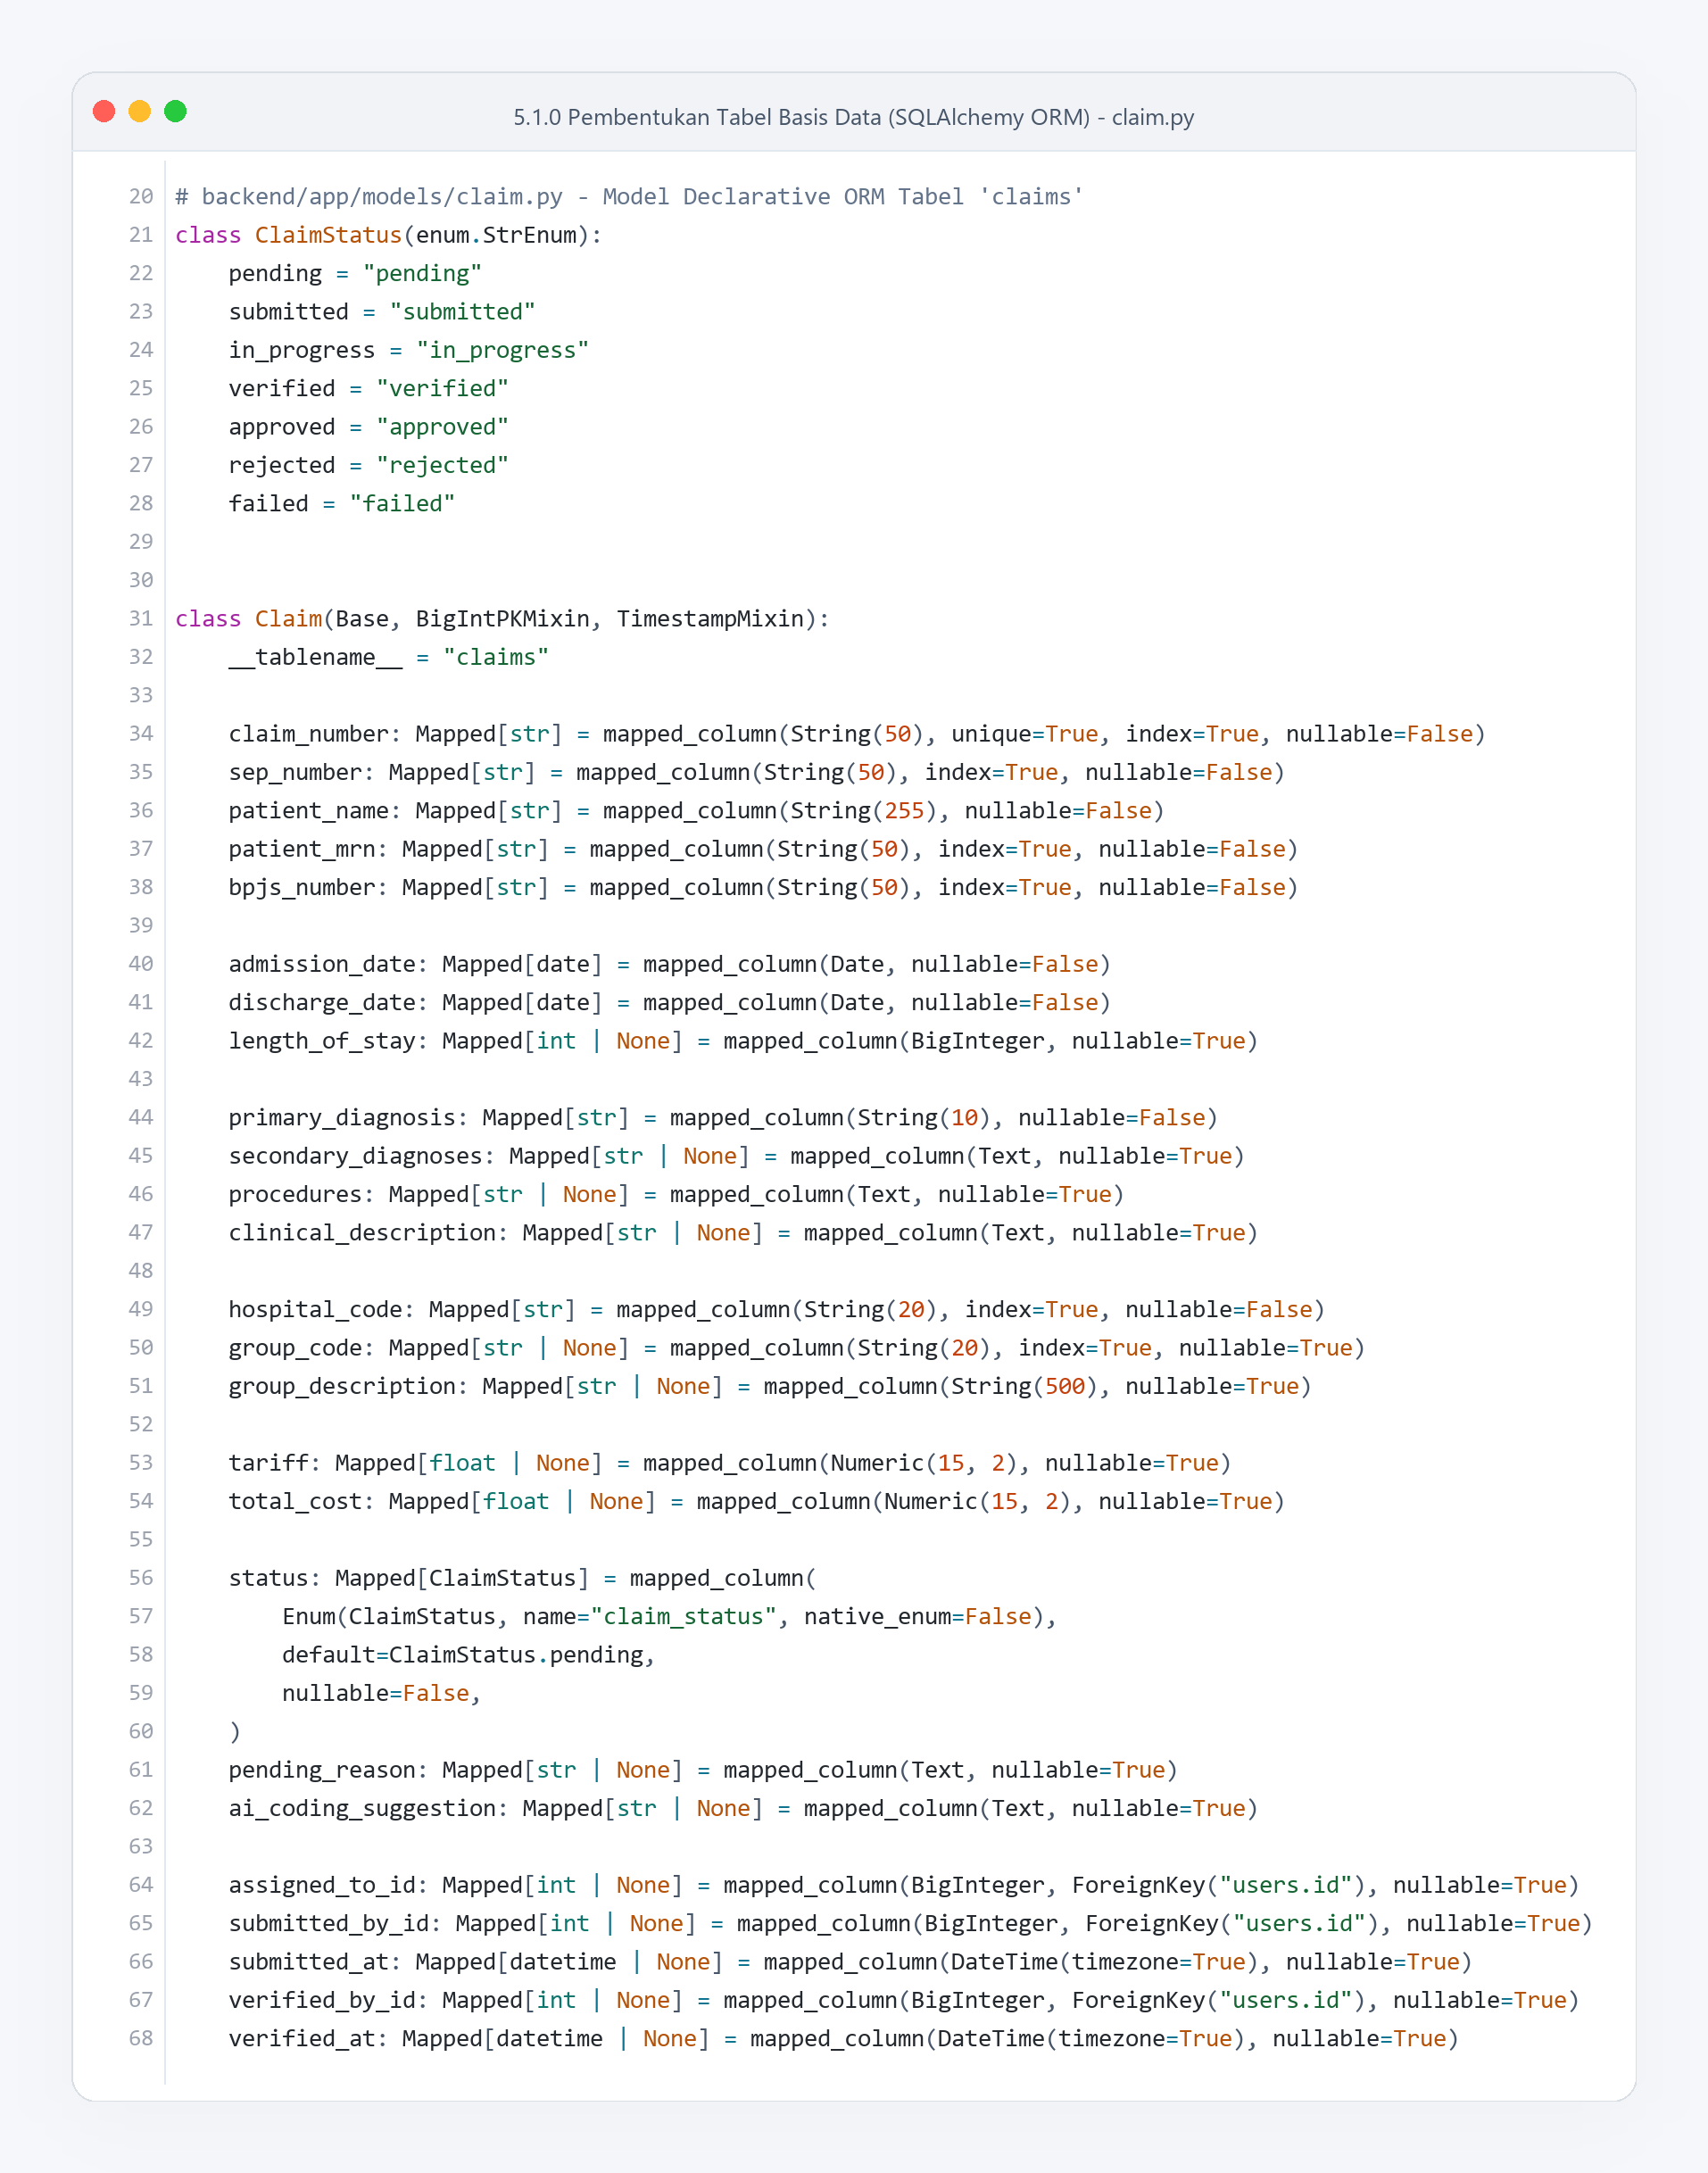
\includegraphics[width=10.5cm]{figure/code/5.1.0_Pembentukan_Tabel_Database.png}
  \caption{Implementasi Model Deklaratif Tabel Claims dengan SQLAlchemy ORM}\label{fig:impl-code-db-models}
\end{figure}

Gambar~\ref{fig:impl-code-db-models} memperlihatkan struktur kelas Claim yang mewarisi kelas dasar Base serta mixin BigIntPKMixin dan TimestampMixin. Entitas ini memuat kolom nomor klaim unik (claim\_number) dan nomor SEP (sep\_number) yang dilengkapi indeks penelusuran cepat. Kolom data identitas pasien mencakup nama pasien, nomor rekam medis, nomor kartu BPJS, serta tanggal masuk dan keluar rawat inap. Pada kolom status klaim, digunakan tipe enumerasi ClaimStatus yang membatasi nilai status ke dalam tujuh kondisi valid: pending, submitted, in\_progress, verified, approved, rejected, dan failed. Penulis merancang alur transisi status ini secara berurutan agar setiap berkas klaim memiliki tahapan pemrosesan yang terdefinisi dengan tegas, serta menolak perubahan data secara sepihak apabila klaim telah mencapai status persetujuan akhir.

Entitas klaim juga menampung atribut data klinis, hasil pengelompokan tarif grouper (group\_code dan tariff), alasan penolakan berkas, serta relasi kunci asing ke tabel pengguna untuk penugasan koder (assigned\_to\_id) dan verifikator (verified\_by\_id). Penulis menerapkan konstrain integritas relasional cascade pada tabel turunan seperti claim\_documents dan claim\_codes, sehingga seluruh data turunan yang terasosiasi dengan berkas klaim akan dikelola secara konsisten tanpa meninggalkan rekaman data yatim (orphaned records) di dalam basis data.

Perubahan skema basis data dikelola secara terkontrol menggunakan alat migrasi Alembic pada berkas migrasi backend/alembic/versions/a8b481027531\_init\_tables.py, seperti ditunjukkan pada Gambar~\ref{fig:impl-code-db-alembic}.

\begin{figure}[!ht]
  \centering
  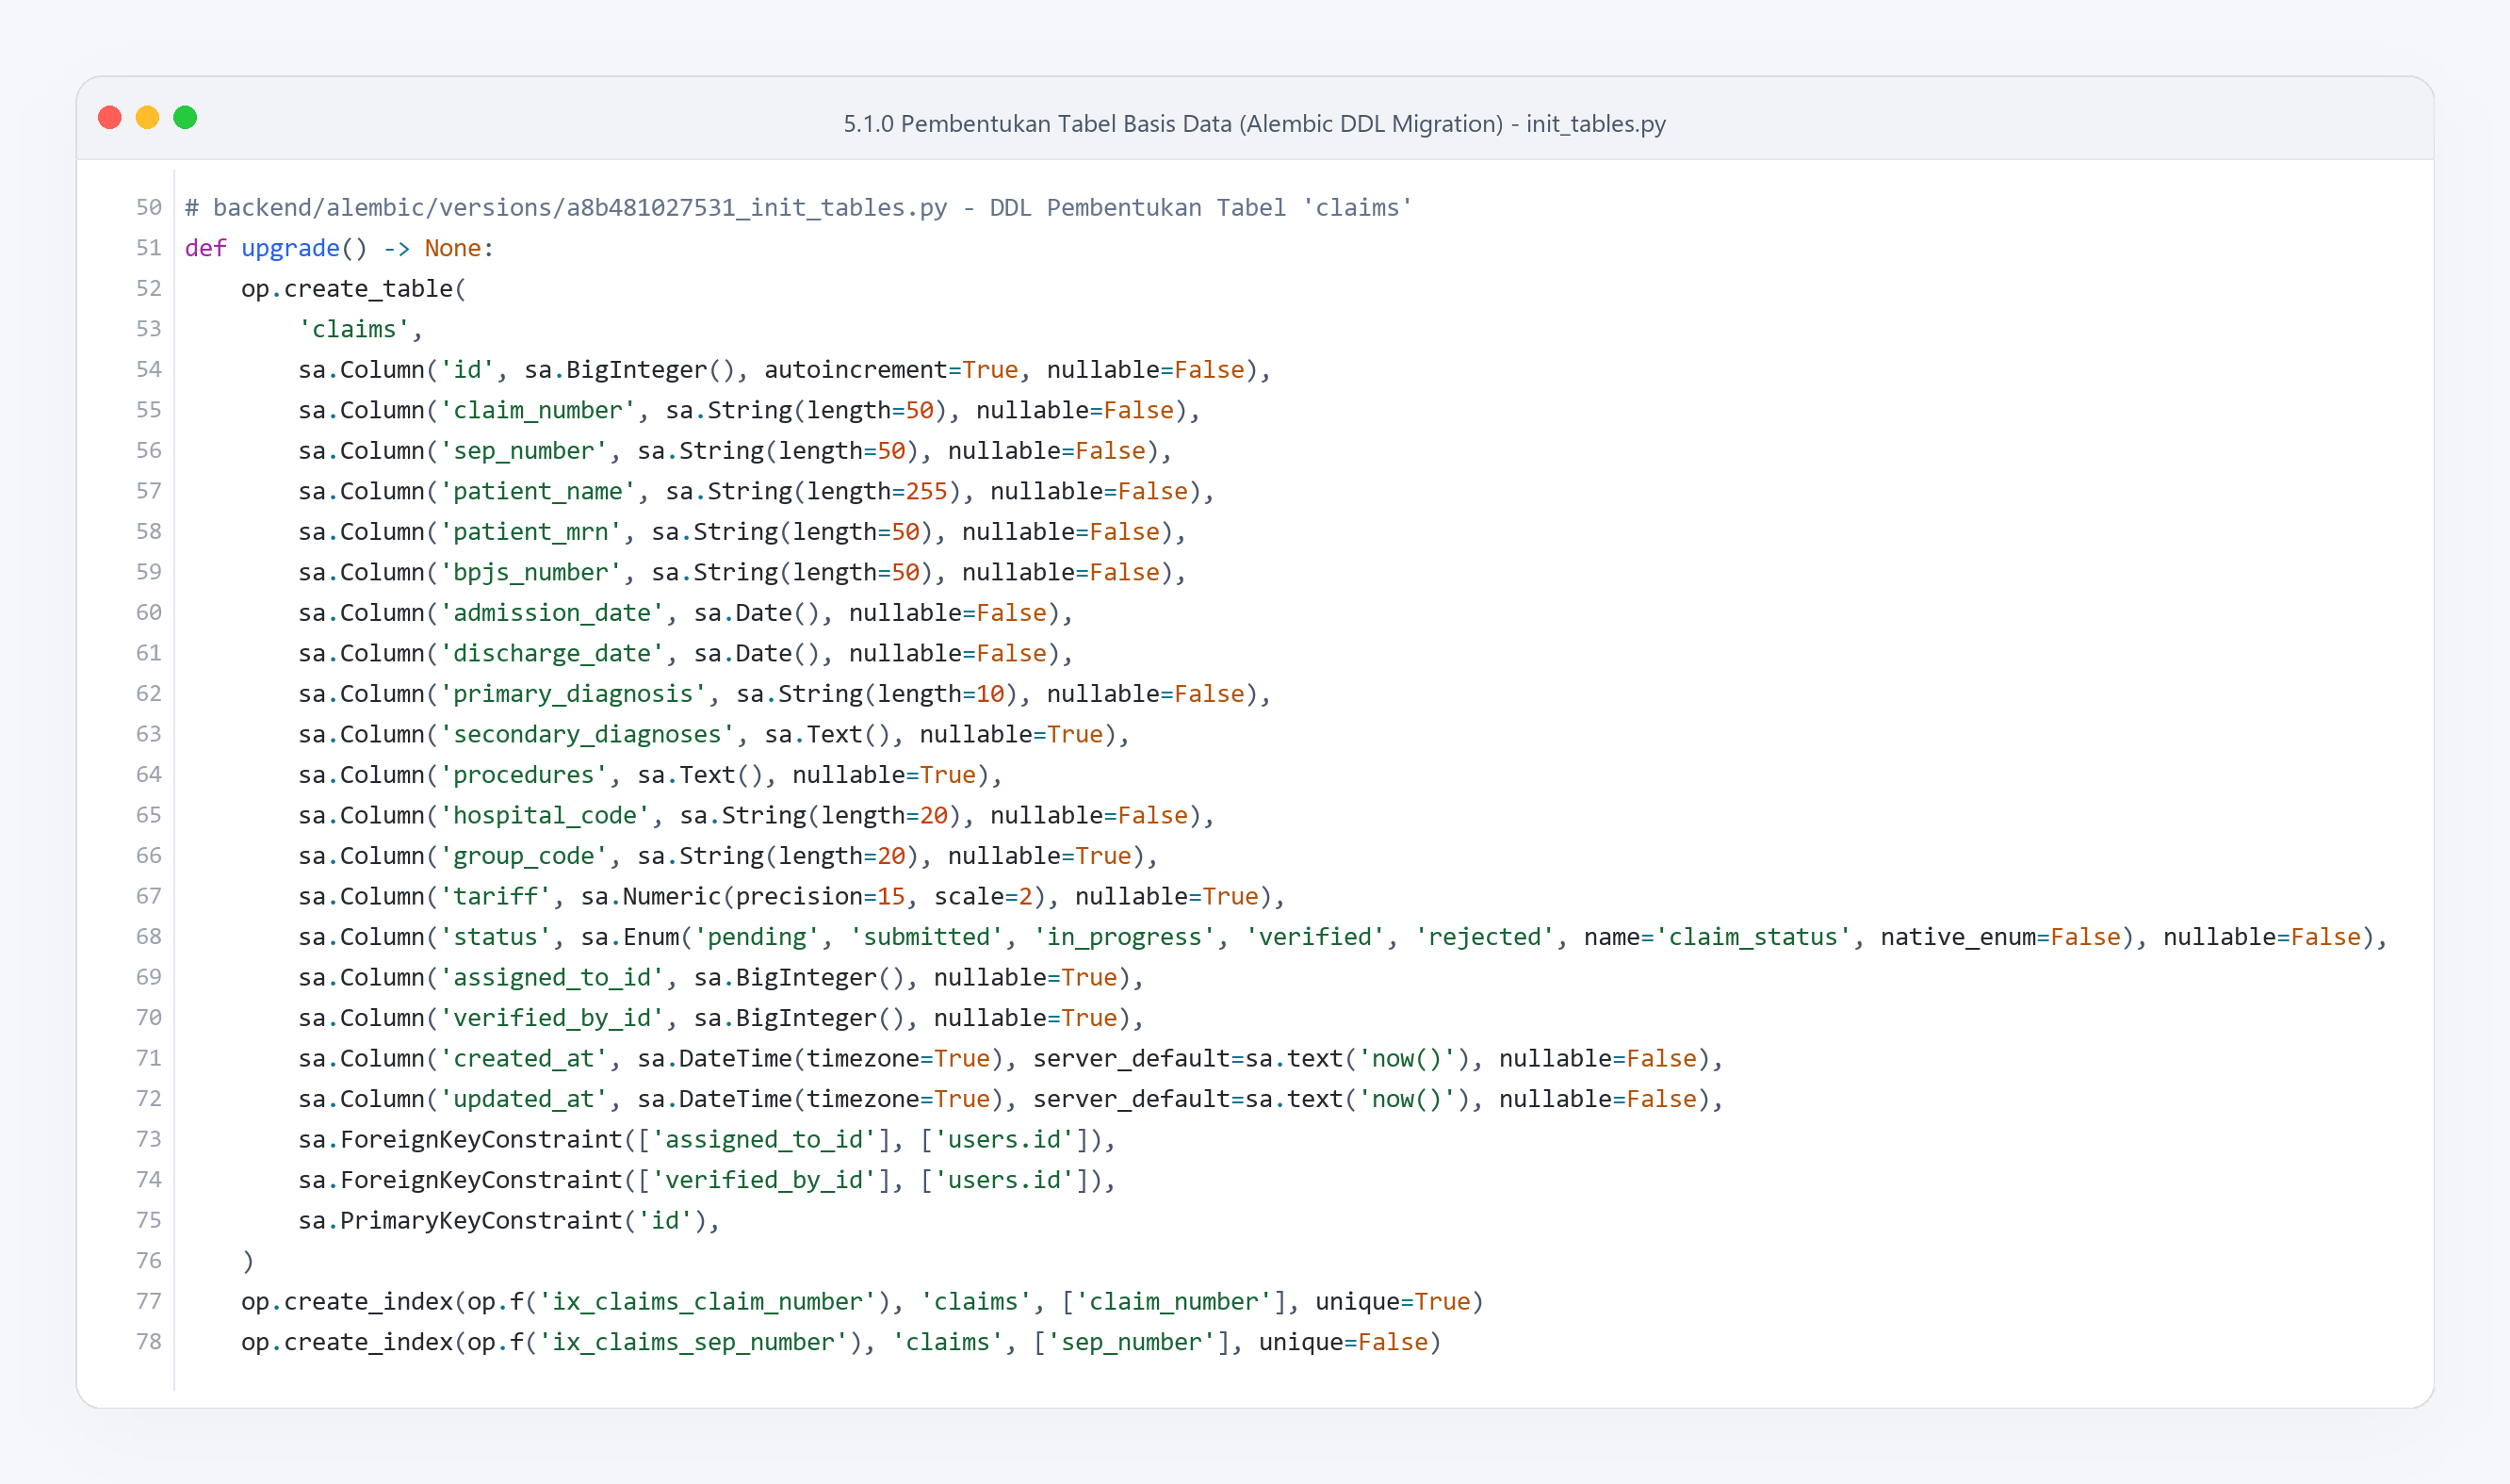
\includegraphics[width=12cm]{figure/code/5.1.0_Pembentukan_Tabel_Database_Alembic.png}
  \caption{Skrip Migrasi DDL Pembentukan Tabel Claims Menggunakan Alembic}\label{fig:impl-code-db-alembic}
\end{figure}

Gambar~\ref{fig:impl-code-db-alembic} memperlihatkan implementasi fungsi upgrade() yang mengeksekusi instruksi Data Definition Language (DDL) op.create\_table() untuk membentuk tabel claims secara fisik di PostgreSQL. Skrip mendefinisikan tipe data presisi tinggi seperti Numeric(15, 2) untuk kolom tarif klaim, penetapan nilai bawaan stempel waktu server\_default=sa.text('now()'), serta deklarasi konstrain integritas data ForeignKeyConstraint ke tabel users. Pada bagian akhir skrip, dibuat indeks unik op.create\_index() pada kolom claim\_number dan indeks sekunder pada sep\_number untuk menjamin kecepatan kueri penelusuran klaim berstatus aktif. Eksekusi migrasi ini diintegrasikan langsung ke dalam alur penerapan sistem menggunakan perintah alembic upgrade head, yang menjamin eksekusi DDL berjalan secara transaksional sehingga kegagalan skema di tengah jalan akan dibatalkan secara otomatis.

\subsection{Modul Autentikasi dan Manajemen Pengguna}
Implementasi logika autentikasi dan manajemen sesi pengguna dibangun pada berkas backend/app/api/v1/auth.py dengan menerapkan protokol OAuth2 dan penerbitan token JSON Web Token (JWT), sebagaimana disajikan pada Gambar~\ref{fig:impl-code-auth}.

\begin{figure}[!ht]
  \centering
  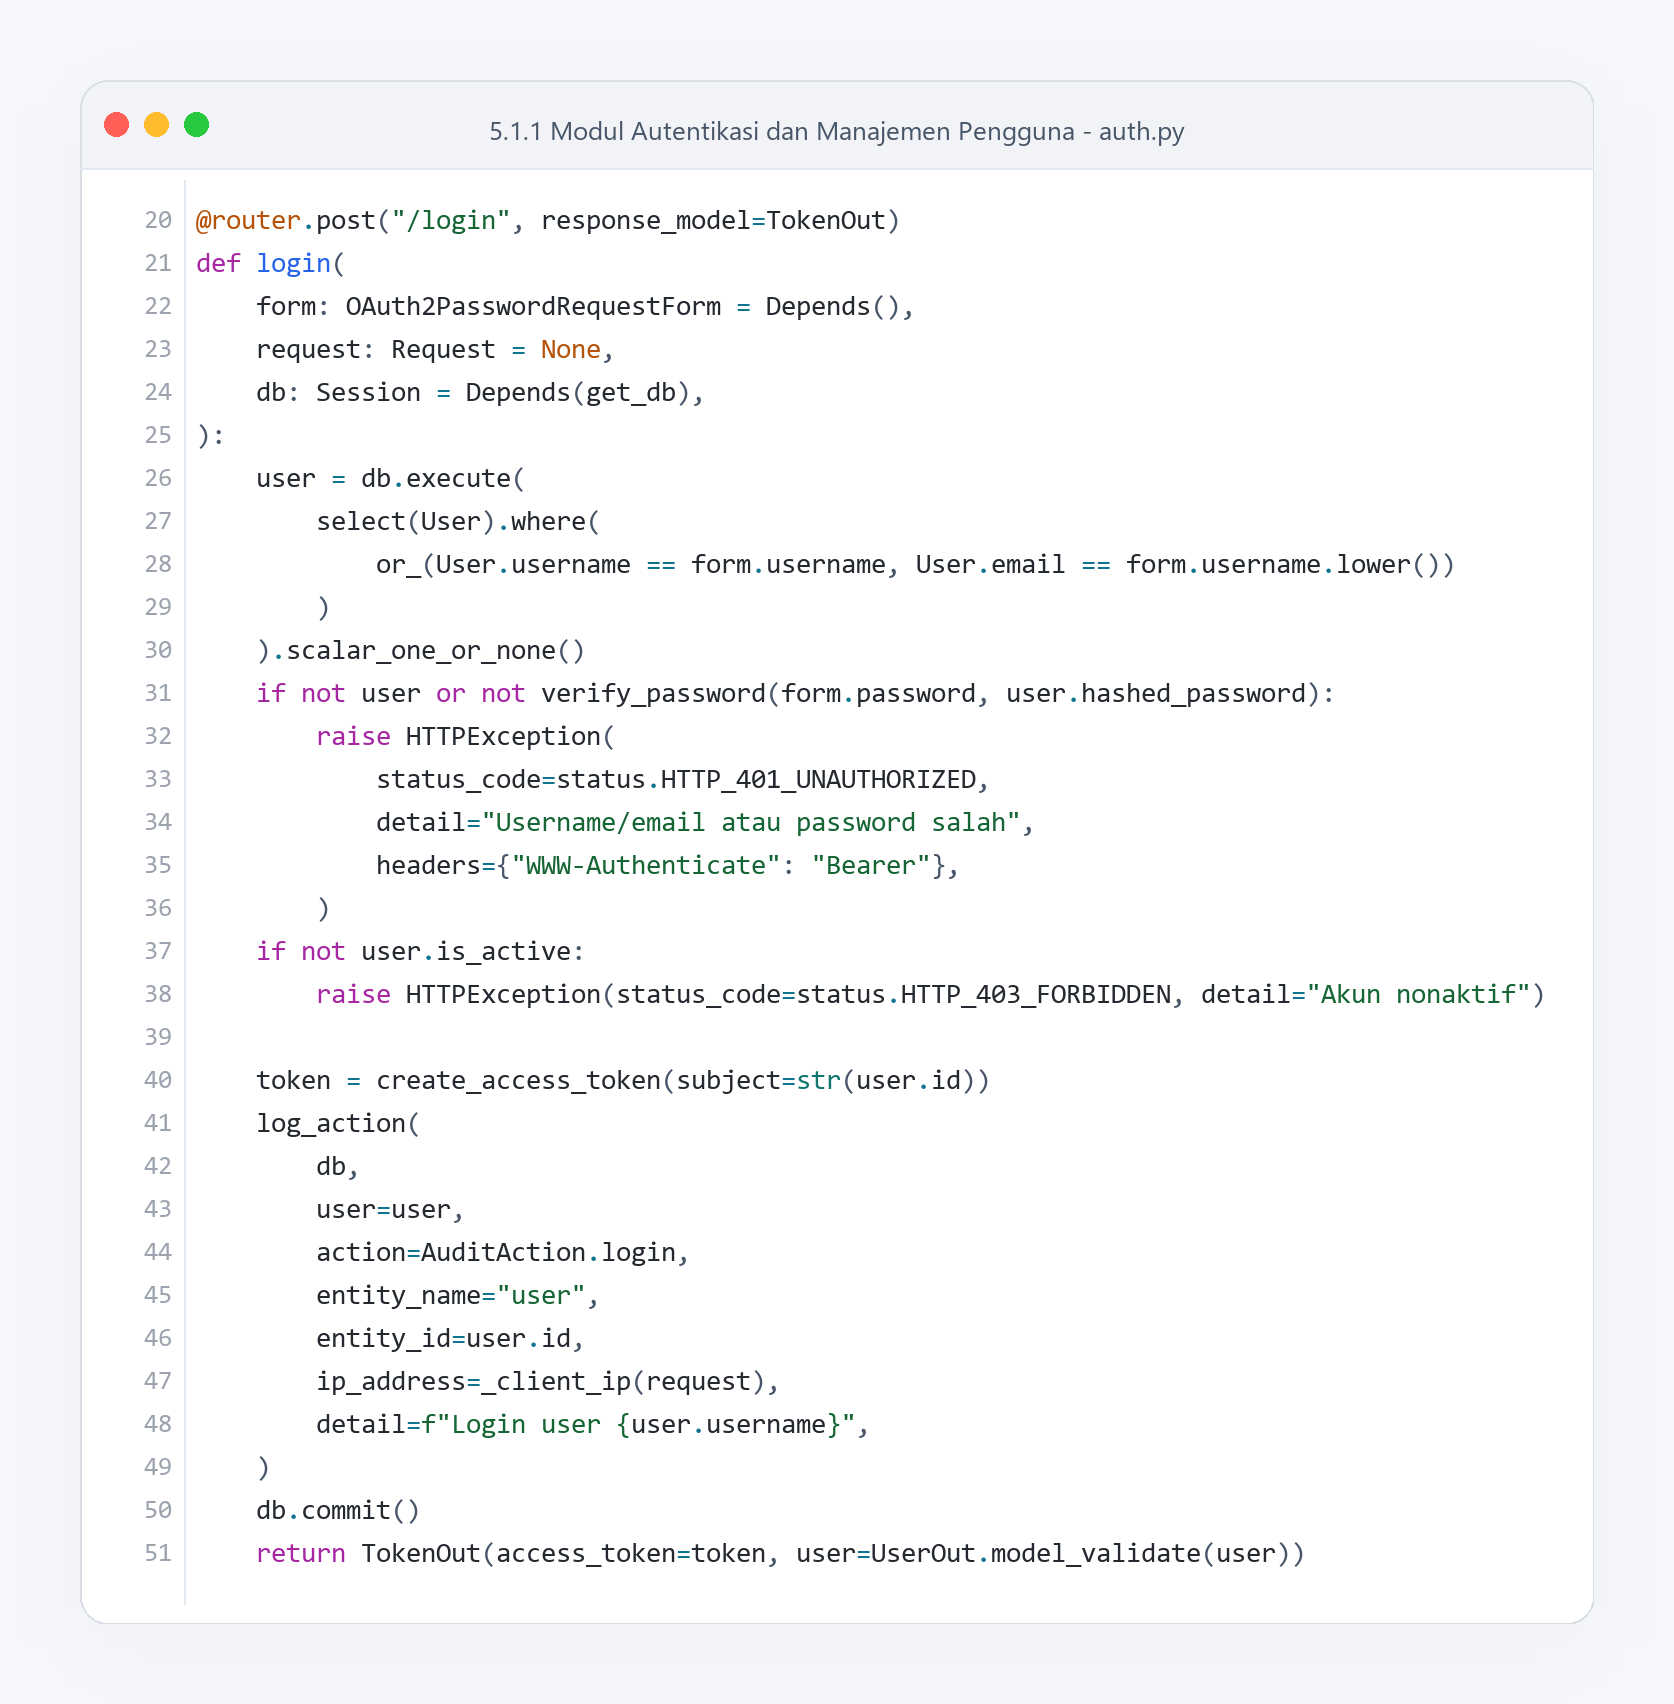
\includegraphics[width=11cm]{figure/code/5.1.1_Modul_Autentikasi_dan_Manajemen_Pengguna.png}
  \caption{Implementasi Endpoint Autentikasi Pengguna dan Penerbitan Token JWT}\label{fig:impl-code-auth}
\end{figure}

Gambar~\ref{fig:impl-code-auth} menguraikan alur kerja fungsi login() pada endpoint POST /login. Sistem menerima kredensial pengguna melalui skema OAuth2PasswordRequestForm dan mencari entitas pengguna di basis data dengan mencocokkan nama pengguna atau alamat surel. Keabsahan kata sandi diuji melalui fungsi verify\_password() yang membandingkan teks masukan terhadap hash aman bcrypt dengan faktor biaya (cost factor) 12 putaran guna mengamankan kredensial dari ancaman brute-force. Apabila kredensial tidak sesuai atau akun berstatus nonaktif, sistem secara tegas melempar eksepsi HTTP 401 Unauthorized atau HTTP 403 Forbidden.

Pengguna yang berhasil diautentikasi akan diterbitkan token akses JWT melalui create\_access\_token(), yang memuat payload terenkripsi berupa identitas pengguna, hak peran, serta masa kedaluwarsa token. Hak akses endpoint privat dikendalikan menggunakan injeksi dependensi FastAPI melalui fungsi get\_current\_active\_user() dan pemilah peran require\_roles(), yang memisahkan hak akses peran koder, verifikator, administrator, dan auditor. Setiap transaksi login yang berhasil maupun yang gagal dicatat secara otomatis ke dalam tabel audit\_logs menggunakan fungsi log\_action() sebelum respon TokenOut dikembalikan ke klien.

\subsection{Modul Manajemen Klaim}
Layanan pengelolaan berkas klaim dan penanganan pengunggahan dokumen resume medis pasien diimplementasikan pada berkas backend/app/api/v1/claims.py, sebagaimana diilustrasikan pada Gambar~\ref{fig:impl-code-claim}.

\begin{figure}[!ht]
  \centering
  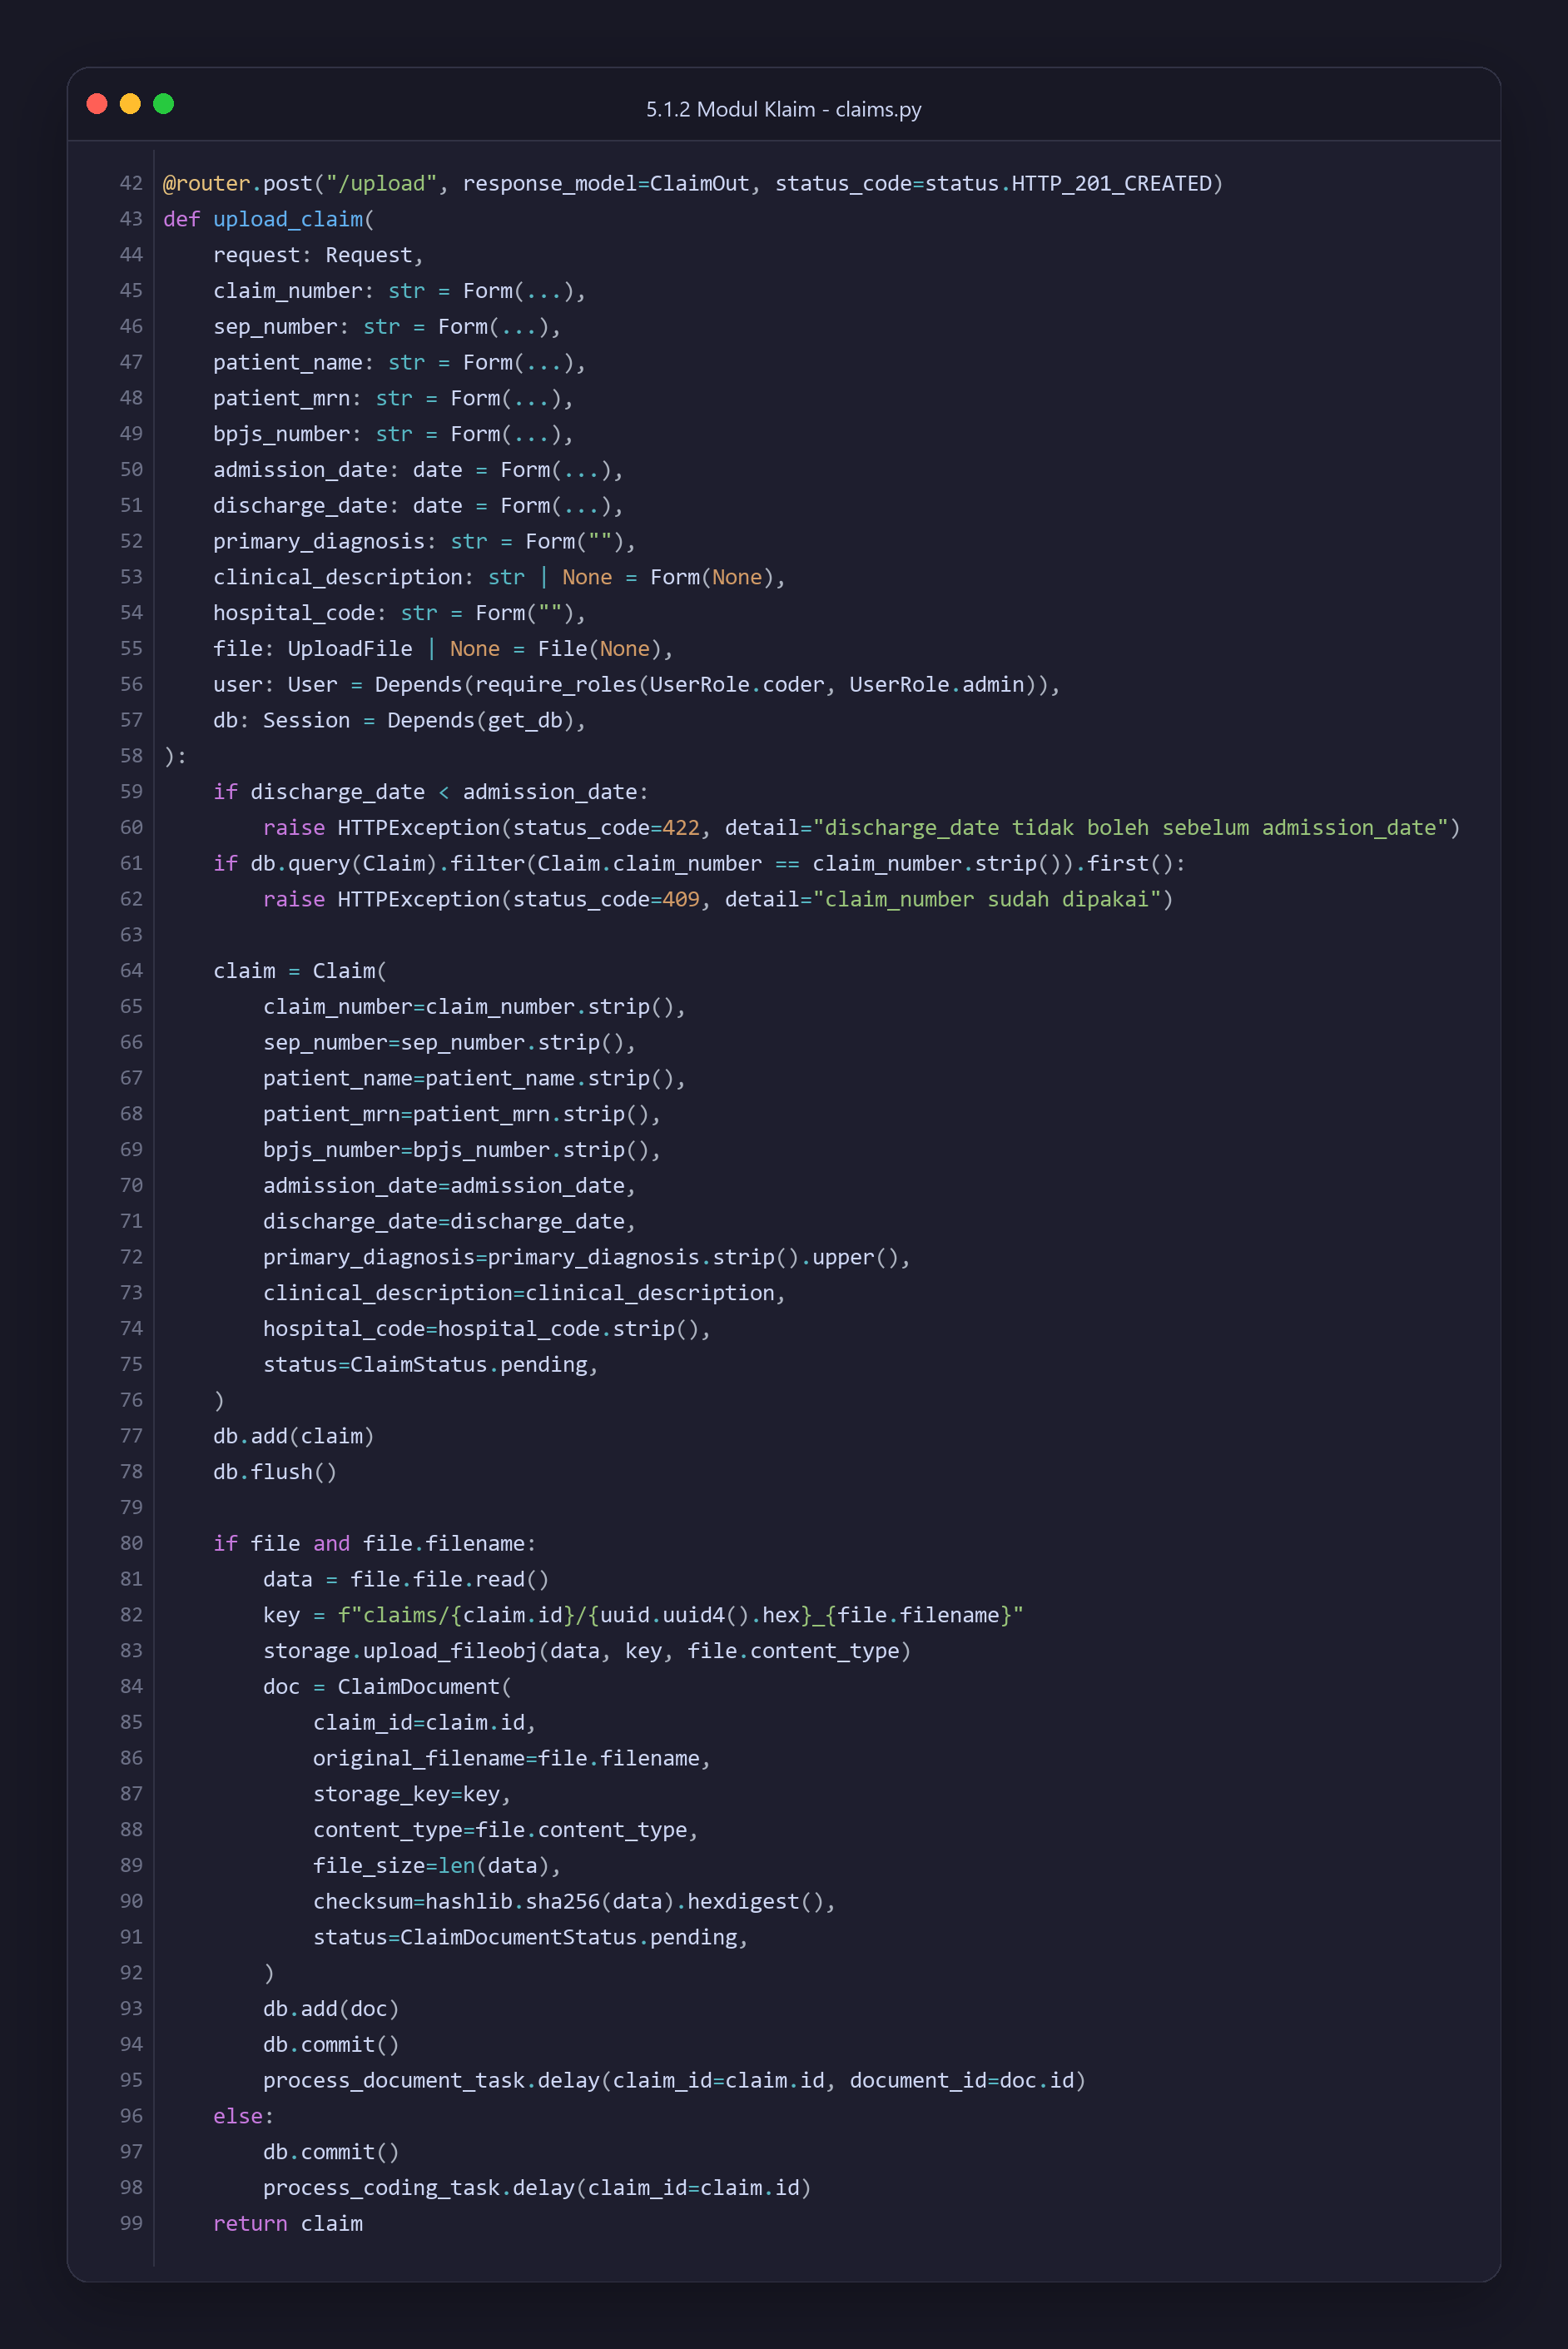
\includegraphics[width=9.5cm]{figure/code/5.1.2_Modul_Klaim.png}
  \caption{Implementasi Endpoint Pengunggahan Berkas Klaim dan Integrasi Penyimpanan}\label{fig:impl-code-claim}
\end{figure}

Gambar~\ref{fig:impl-code-claim} memperlihatkan fungsi upload\_claim() pada endpoint POST /upload yang dilindungi otorisasi peran koder dan admin. Sistem menerapkan aturan validasi bisnis dengan memeriksa bahwa tanggal keluar perawatan tidak boleh mendahului tanggal masuk rawat, serta mencegah duplikasi nomor klaim yang telah terdaftar di basis data dengan respon HTTP 409 Conflict. Berkas fisik resume medis yang diunggah dibaca secara biner dalam potongan memori (stream chunk) guna mencegah lonjakan penggunaan memori peladen saat menangani berkas rekam medis berukuran besar. Berkas tersebut kemudian diberikan kunci penyimpanan unik berbasis UUID dan ditransfer ke penyimpanan objek Cloudflare R2 melalui fungsi storage.upload\_fileobj() yang menggunakan protokol S3-compatible.

Untuk menjamin integritas data resume medis terhadap risiko kerusakan berkas atau manipulasi pihak tidak berwenang, sistem menghitung nilai hash SHA-256 dari berkas dokumen sebelum disimpan. Seluruh rangkaian proses pencatatan data klaim, penyimpanan metadata berkas ke tabel claim\_documents dengan status pending, serta pemicuan tugas pemrosesan latar belakang Celery melalui pemanggilan process\_document\_task.delay() dikemas dalam satu transaksi basis data yang atomik. Pendekatan ini memastikan tidak ada berkas tanpa metadata klaim yang tertinggal di penyimpanan awan jika terjadi kendala jaringan saat pengunggahan.

\subsection{Modul Pemrosesan Dokumen Asinkron}
Tugas pemrosesan komputasi berat untuk mengekstrak informasi teks klinis dari dokumen resume medis dijalankan di latar belakang oleh pekerja Celery pada berkas backend/app/worker/tasks.py, seperti ditunjukkan pada Gambar~\ref{fig:impl-code-doc-worker}.

\begin{figure}[!ht]
  \centering
  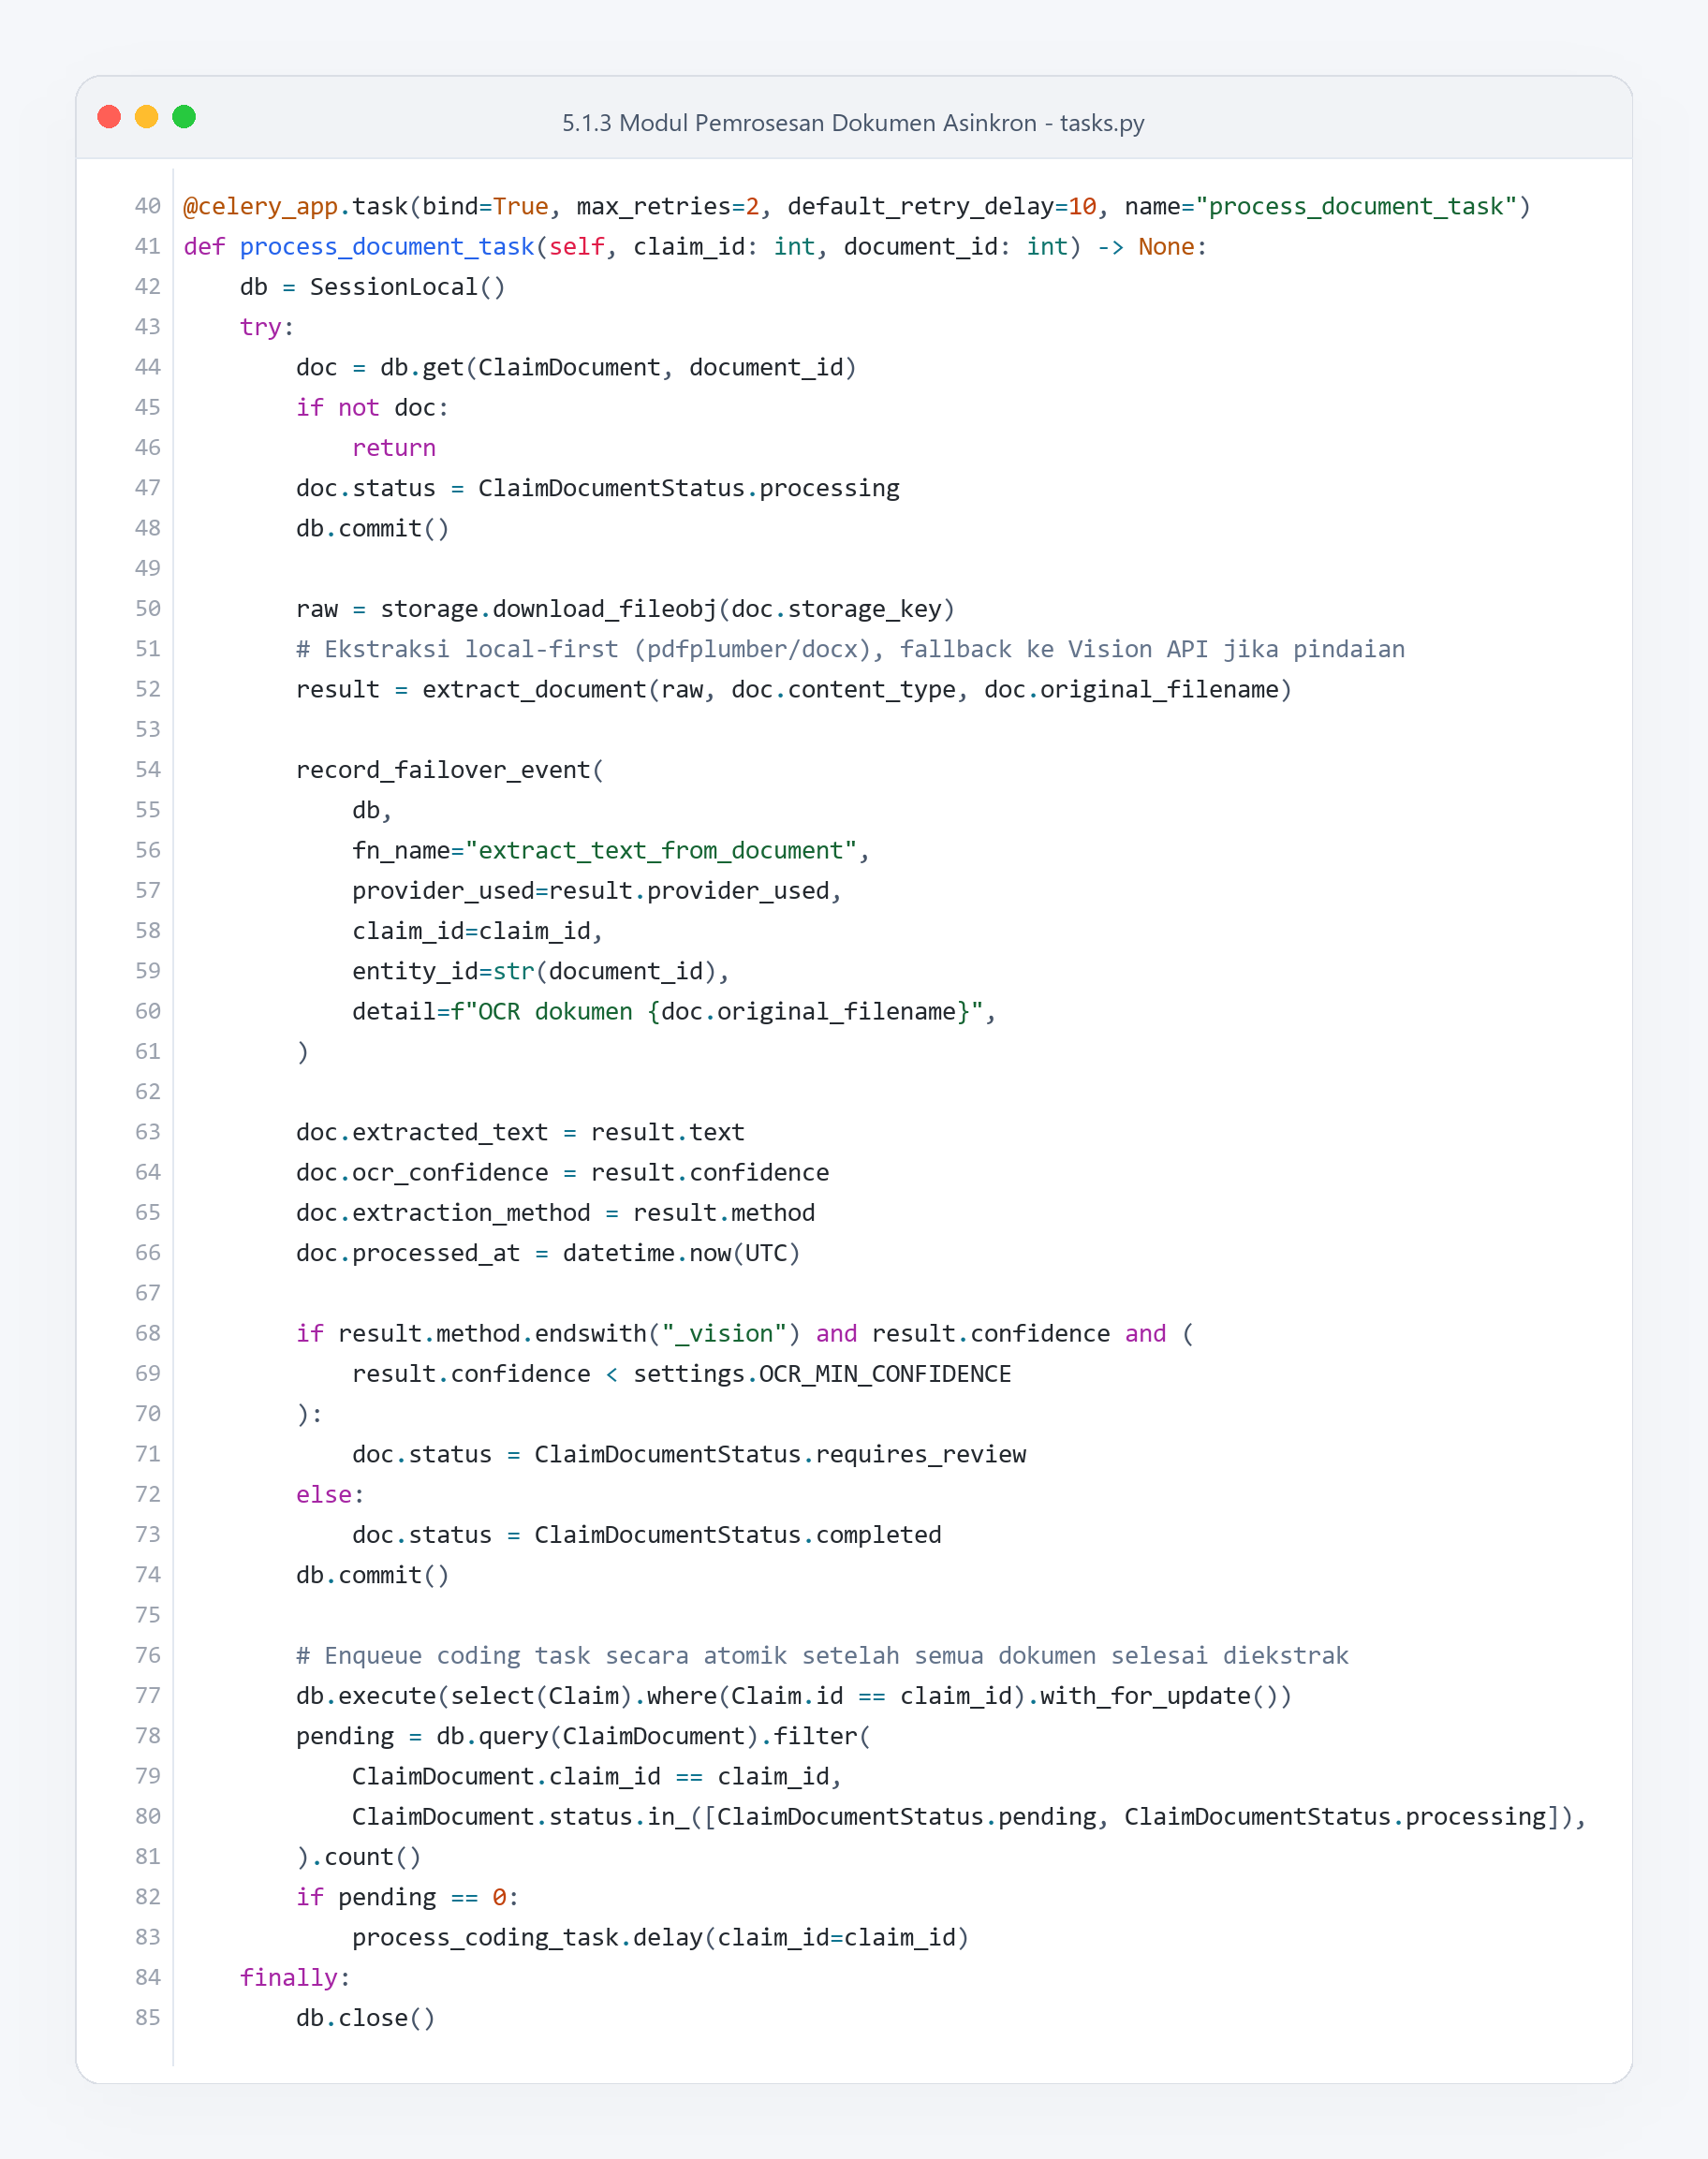
\includegraphics[width=10.5cm]{figure/code/5.1.3_Modul_Pemrosesan_Dokumen_Asinkron.png}
  \caption{Implementasi Tugas Pekerja Celery untuk Ekstraksi Dokumen Medis}\label{fig:impl-code-doc-worker}
\end{figure}

Gambar~\ref{fig:impl-code-doc-worker} menampilkan fungsi tugas process\_document\_task() yang dikonfigurasi dengan batas percobaan ulang otomatis (max\_retries=2) dan jeda eksponensial (exponential backoff). Pekerja Celery mengunduh berkas dari Cloudflare R2 dan mengekstrak teks menggunakan pendekatan lokal (local-first) dengan pustaka pdfplumber untuk dokumen PDF dan python-docx untuk berkas Word. Pendekatan lokal ini mempercepat durasi ekstraksi teks hingga di bawah dua detik untuk berkas standar serta menghemat pemakaian kuota API eksternal.

Apabila berkas yang diunggah berupa gambar hasil pindaian atau lapisan teks PDF bernilai kosong, sistem secara otomatis mengalihkan proses ekstraksi ke model Vision OCR AI dan mencatat peristiwa pengalihan layanan melalui record\_failover\_event(). Jika skor keyakinan OCR berada di bawah ambang batas minimum 0,70, status dokumen dialihkan menjadi requires\_review agar ditinjau secara manual oleh staf koder. Setelah seluruh berkas milik klaim selesai diekstrak secara lengkap, pekerja Celery secara atomik memperbarui status klaim menjadi in\_progress dan mendaftarkan tugas inferensi koding klinis berikutnya melalui pemanggilan process\_coding\_task.delay().

\subsection{Modul Rekomendasi Koding AI}
Analisis rekam medis dan pemberian rekomendasi kode diagnosis ICD-10 serta prosedur ICD-9-CM diimplementasikan pada berkas backend/app/api/v1/coding.py, sebagaimana disajikan pada Gambar~\ref{fig:impl-code-ai-coding}.

\begin{figure}[!ht]
  \centering
  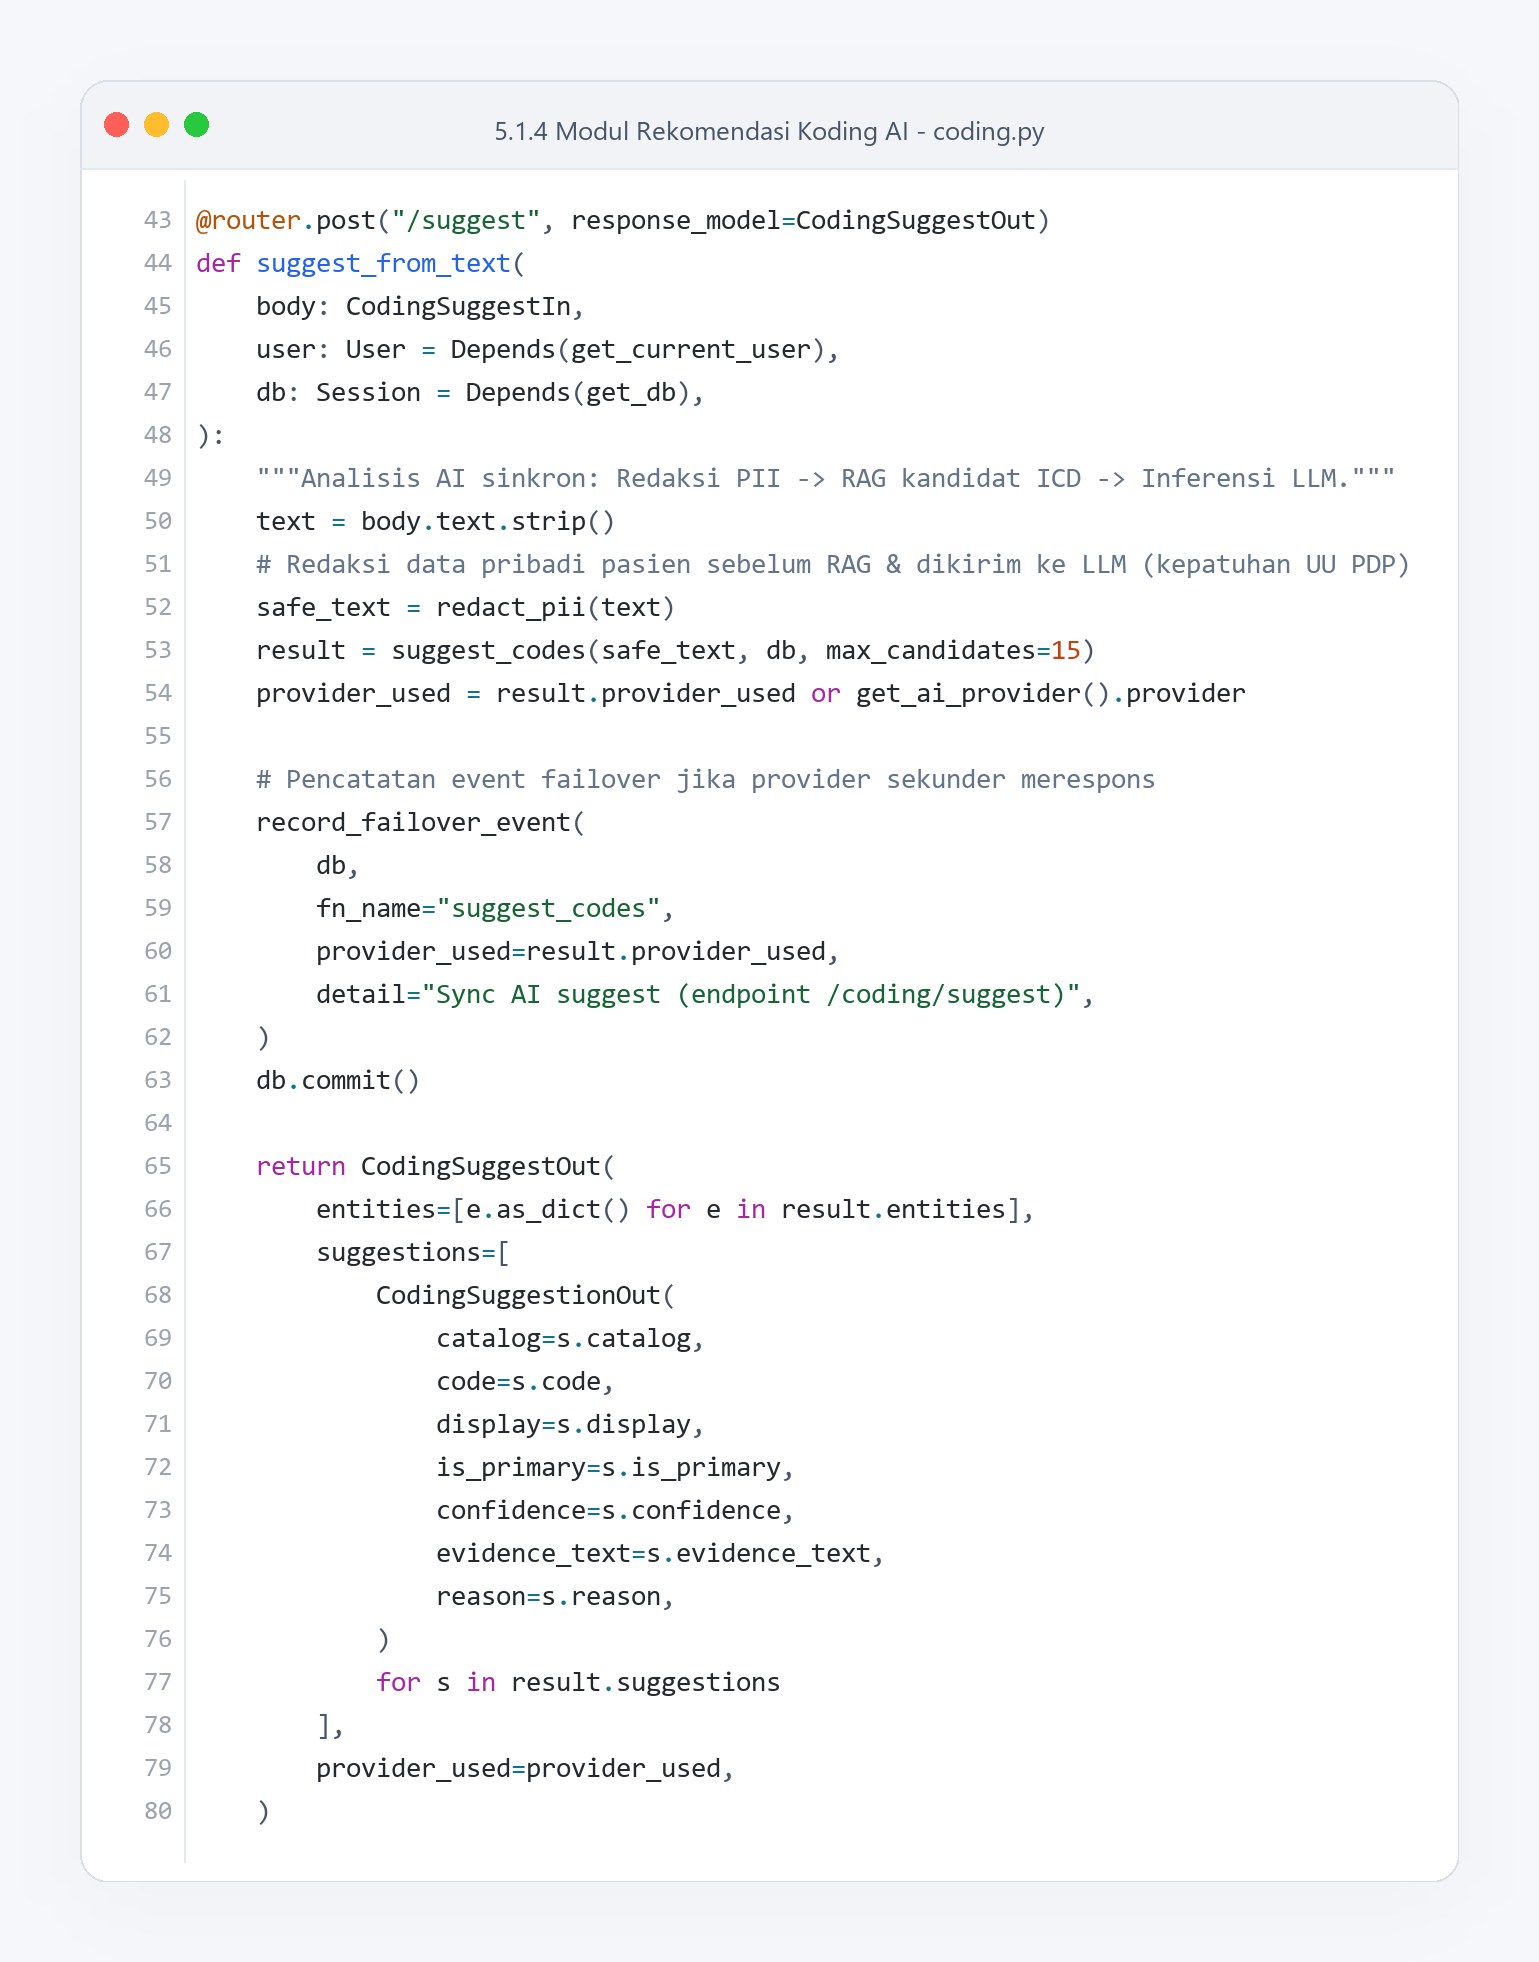
\includegraphics[width=10.5cm]{figure/code/5.1.4_Modul_Rekomendasi_Koding_AI.png}
  \caption{Implementasi Endpoint Rekomendasi Koding AI dan Sanitasi Data Pribadi}\label{fig:impl-code-ai-coding}
\end{figure}

Gambar~\ref{fig:impl-code-ai-coding} memperlihatkan implementasi endpoint POST /suggest pada fungsi suggest\_from\_text(). Sebelum teks rekam medis dikirimkan ke model bahasa besar eksternal, sistem secara otomatis menjalankan fungsi redact\_pii() untuk menyamarkan identitas pribadi pasien (Personally Identifiable Information/PII). Penulis merancang modul penyamaran ini menggunakan pencocokan pola ekspresi reguler terstruktur untuk mendeteksi NIK 16 digit, nomor kartu BPJS Kesehatan 13 digit, nomor rekam medis, tanggal lahir, nama pasien, dan identitas dokter. Langkah ini menjamin kepatuhan penuh terhadap mandat perlindungan kerahasiaan data kesehatan pada UU PDP No. 27 Tahun 2022 dan PMK No. 24 Tahun 2022.

Teks yang telah disanitasi kemudian diproses oleh mesin pencari kandidat RAG dan model AI utama Google Gemini menggunakan instruksi terstruktur (system prompt). Model diarahkan untuk menghasilkan luaran terstruktur berupa skema JSON Pydantic yang memuat usulan kode diagnosis dan prosedur beserta tingkat keyakinan (confidence) dan kutipan bukti teks klinis (evidence\_text). Apabila penyedia utama mengalami kendala batas laju pemanggilan (rate limit HTTP 429) atau batas waktu koneksi terlampaui, sistem secara transparan mengalihkan permintaan ke penyedia cadangan OpenRouter melalui pola circuit breaker dan mencatat insiden pengalihan tersebut ke basis data.

\subsection{Modul Keputusan Koding}
Fungsionalitas bagi petugas koding medis untuk menetapkan keputusan akhir terhadap usulan kode klinis diimplementasikan pada berkas backend/app/api/v1/coding.py, seperti diperlihatkan pada Gambar~\ref{fig:impl-code-decide-codes}.

\begin{figure}[!ht]
  \centering
  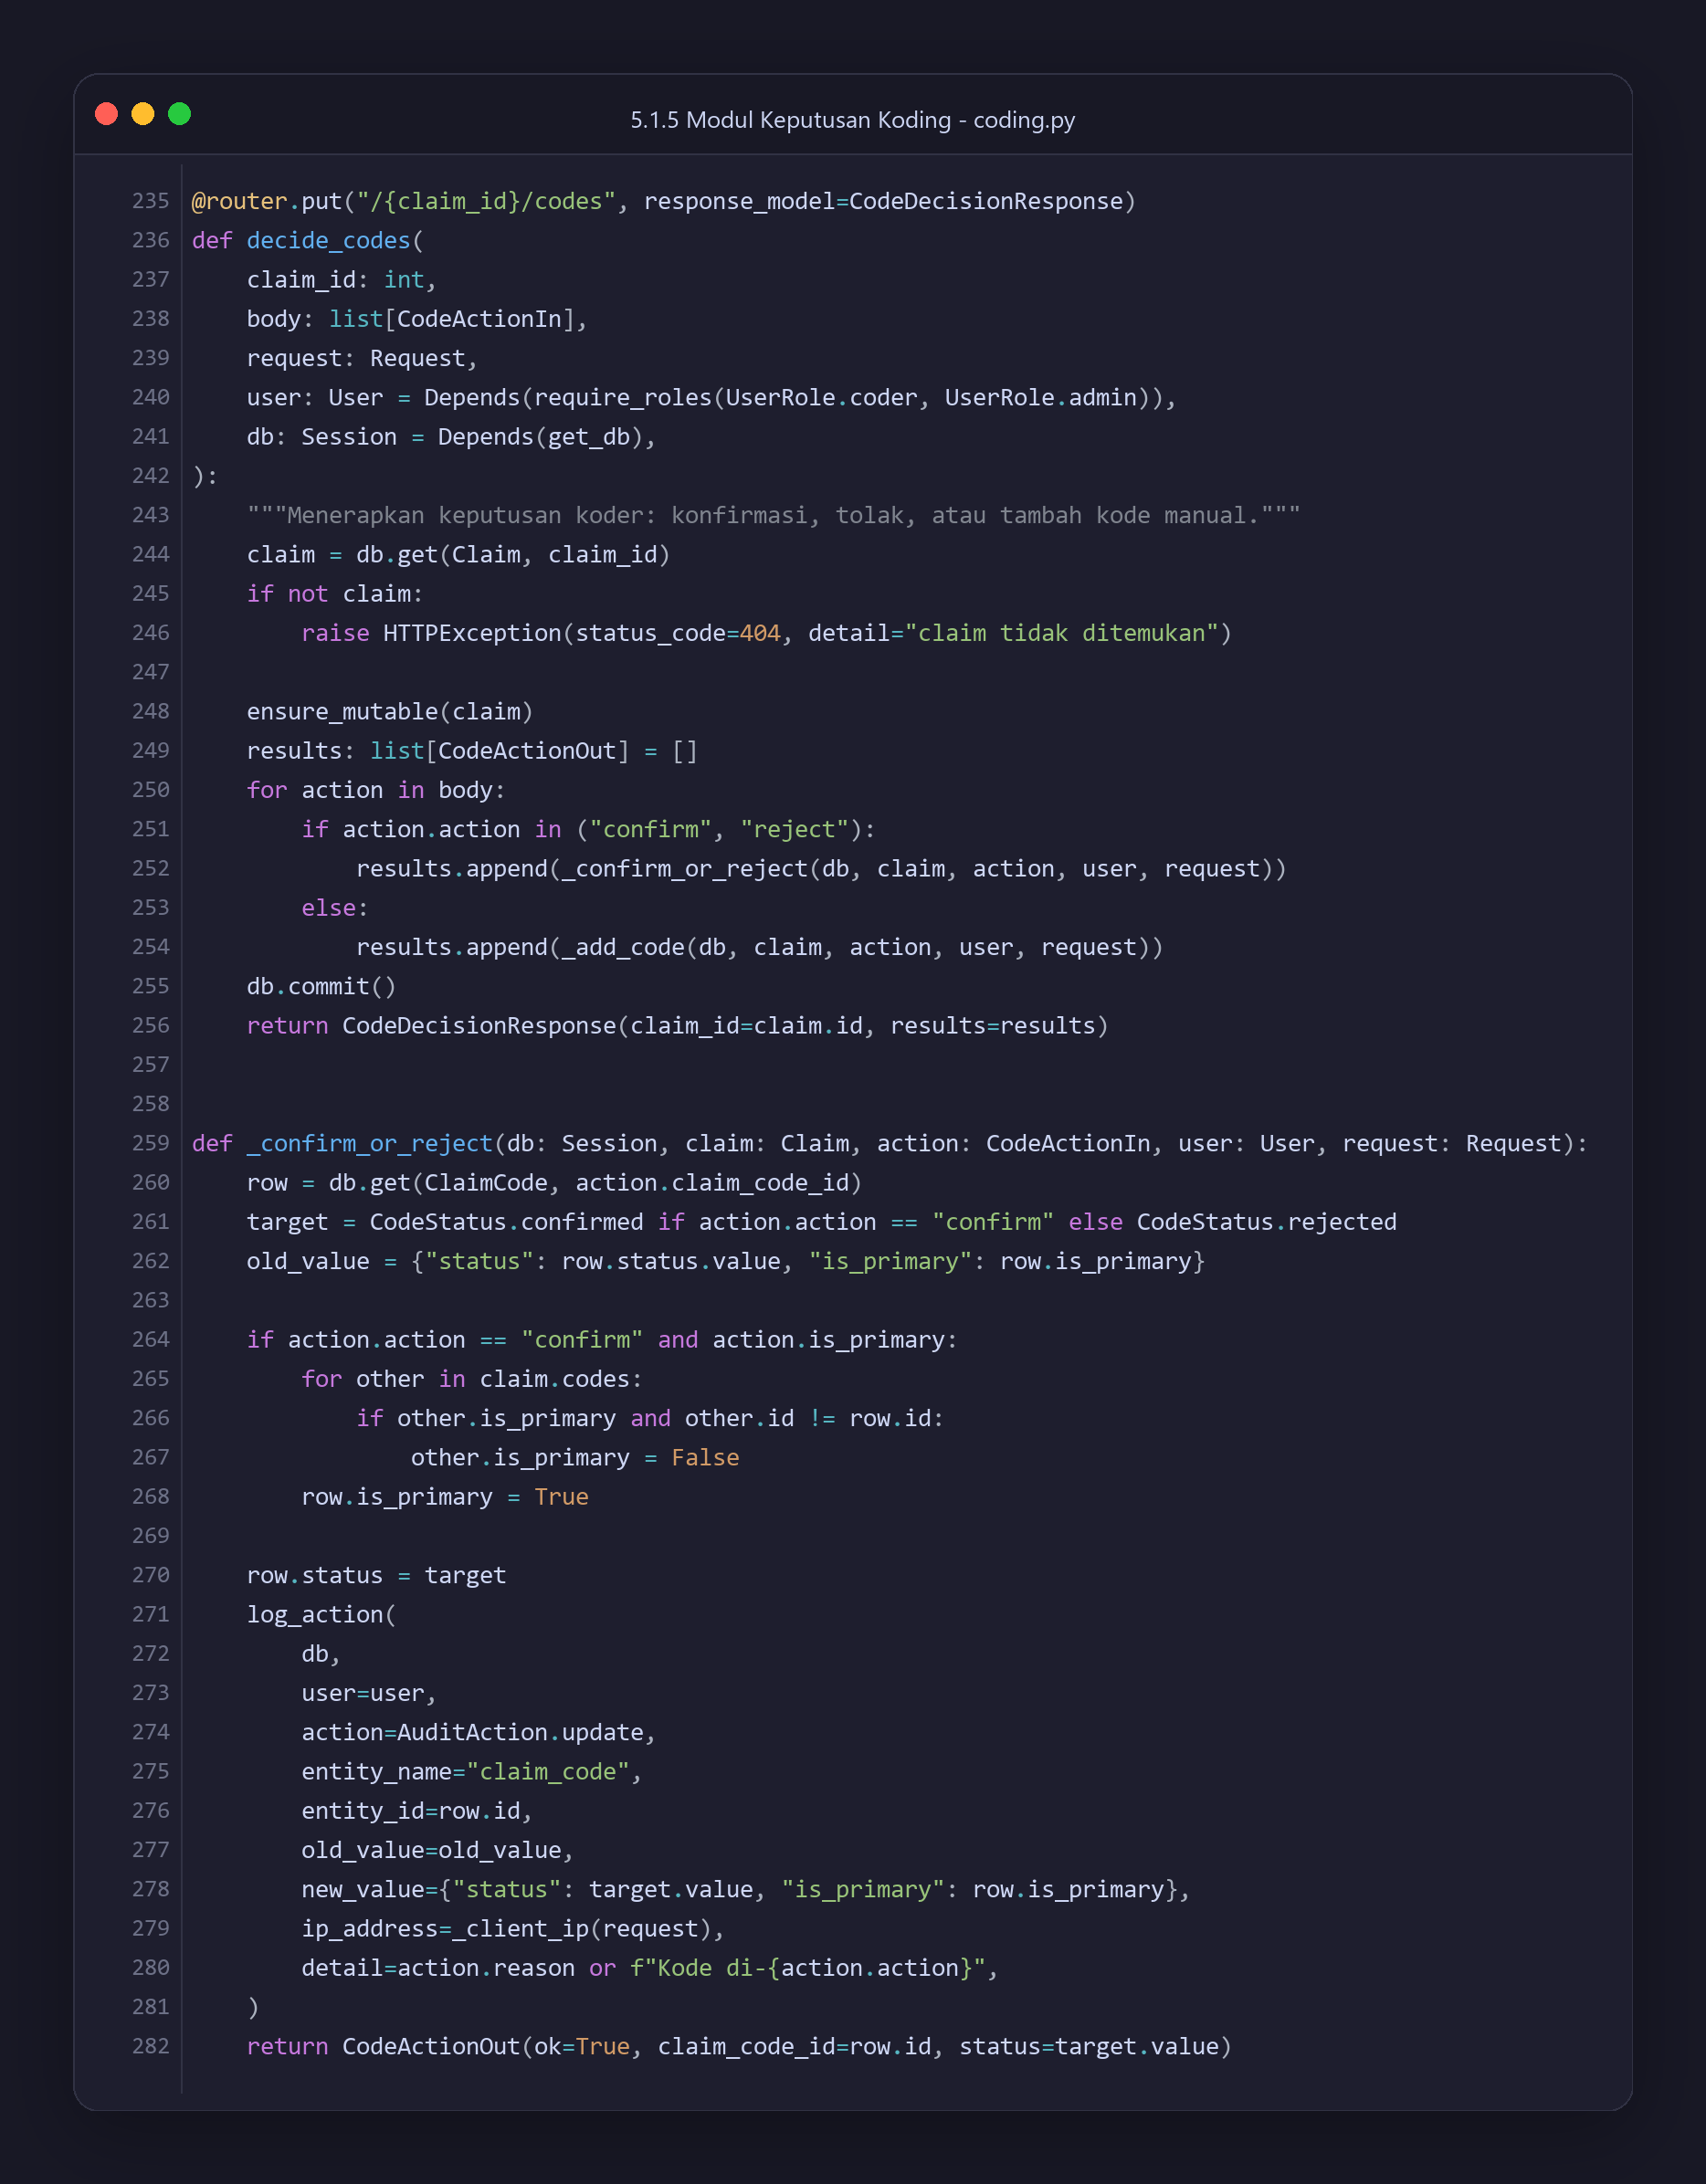
\includegraphics[width=10.5cm]{figure/code/5.1.5_Modul_Keputusan_Koding.png}
  \caption{Implementasi Logika Penetapan Keputusan Koding Medis oleh Koder}\label{fig:impl-code-decide-codes}
\end{figure}

Gambar~\ref{fig:impl-code-decide-codes} menguraikan logika fungsi decide\_codes() pada endpoint PUT /\{claim\_id\}/codes yang mengelola konfirmasi usulan kode, penolakan kode yang tidak sesuai, maupun penambahan kode secara manual dari katalog ICD. Sistem menerapkan aturan bisnis klaim BPJS Kesehatan di mana tepat hanya boleh ada satu diagnosis primer yang aktif pada setiap berkas klaim. Ketika koder menetapkan suatu kode baru sebagai diagnosis primer (is\_primary=True), sistem secara otomatis mengatur penanda primer pada kode diagnosis lain menjadi False melalui pemutakhiran atomik di basis data.

Selain itu, fungsi \_confirm\_or\_reject() memvalidasi kepemilikan kode klaim dan secara konsisten mencatat riwayat perubahan status kode dari kondisi lama (old\_value) ke kondisi baru (new\_value) ke dalam log audit. Pencatatan ini mencakup stempel waktu perubahan dan identitas pengguna pelaksana aksi guna menjamin akuntabilitas koding medis dan memfasilitasi penelusuran jika terjadi audit verifikasi oleh pihak BPJS Kesehatan.

\subsection{Modul Grouper INA-CBG}
Perhitungan kelompok kasus dan estimasi nilai tarif klaim berdasarkan kombinasi kode diagnosis dan prosedur yang telah terkonfirmasi diimplementasikan pada berkas backend/app/api/v1/grouper.py, sebagaimana diilustrasikan pada Gambar~\ref{fig:impl-code-grouper}.

\begin{figure}[!ht]
  \centering
  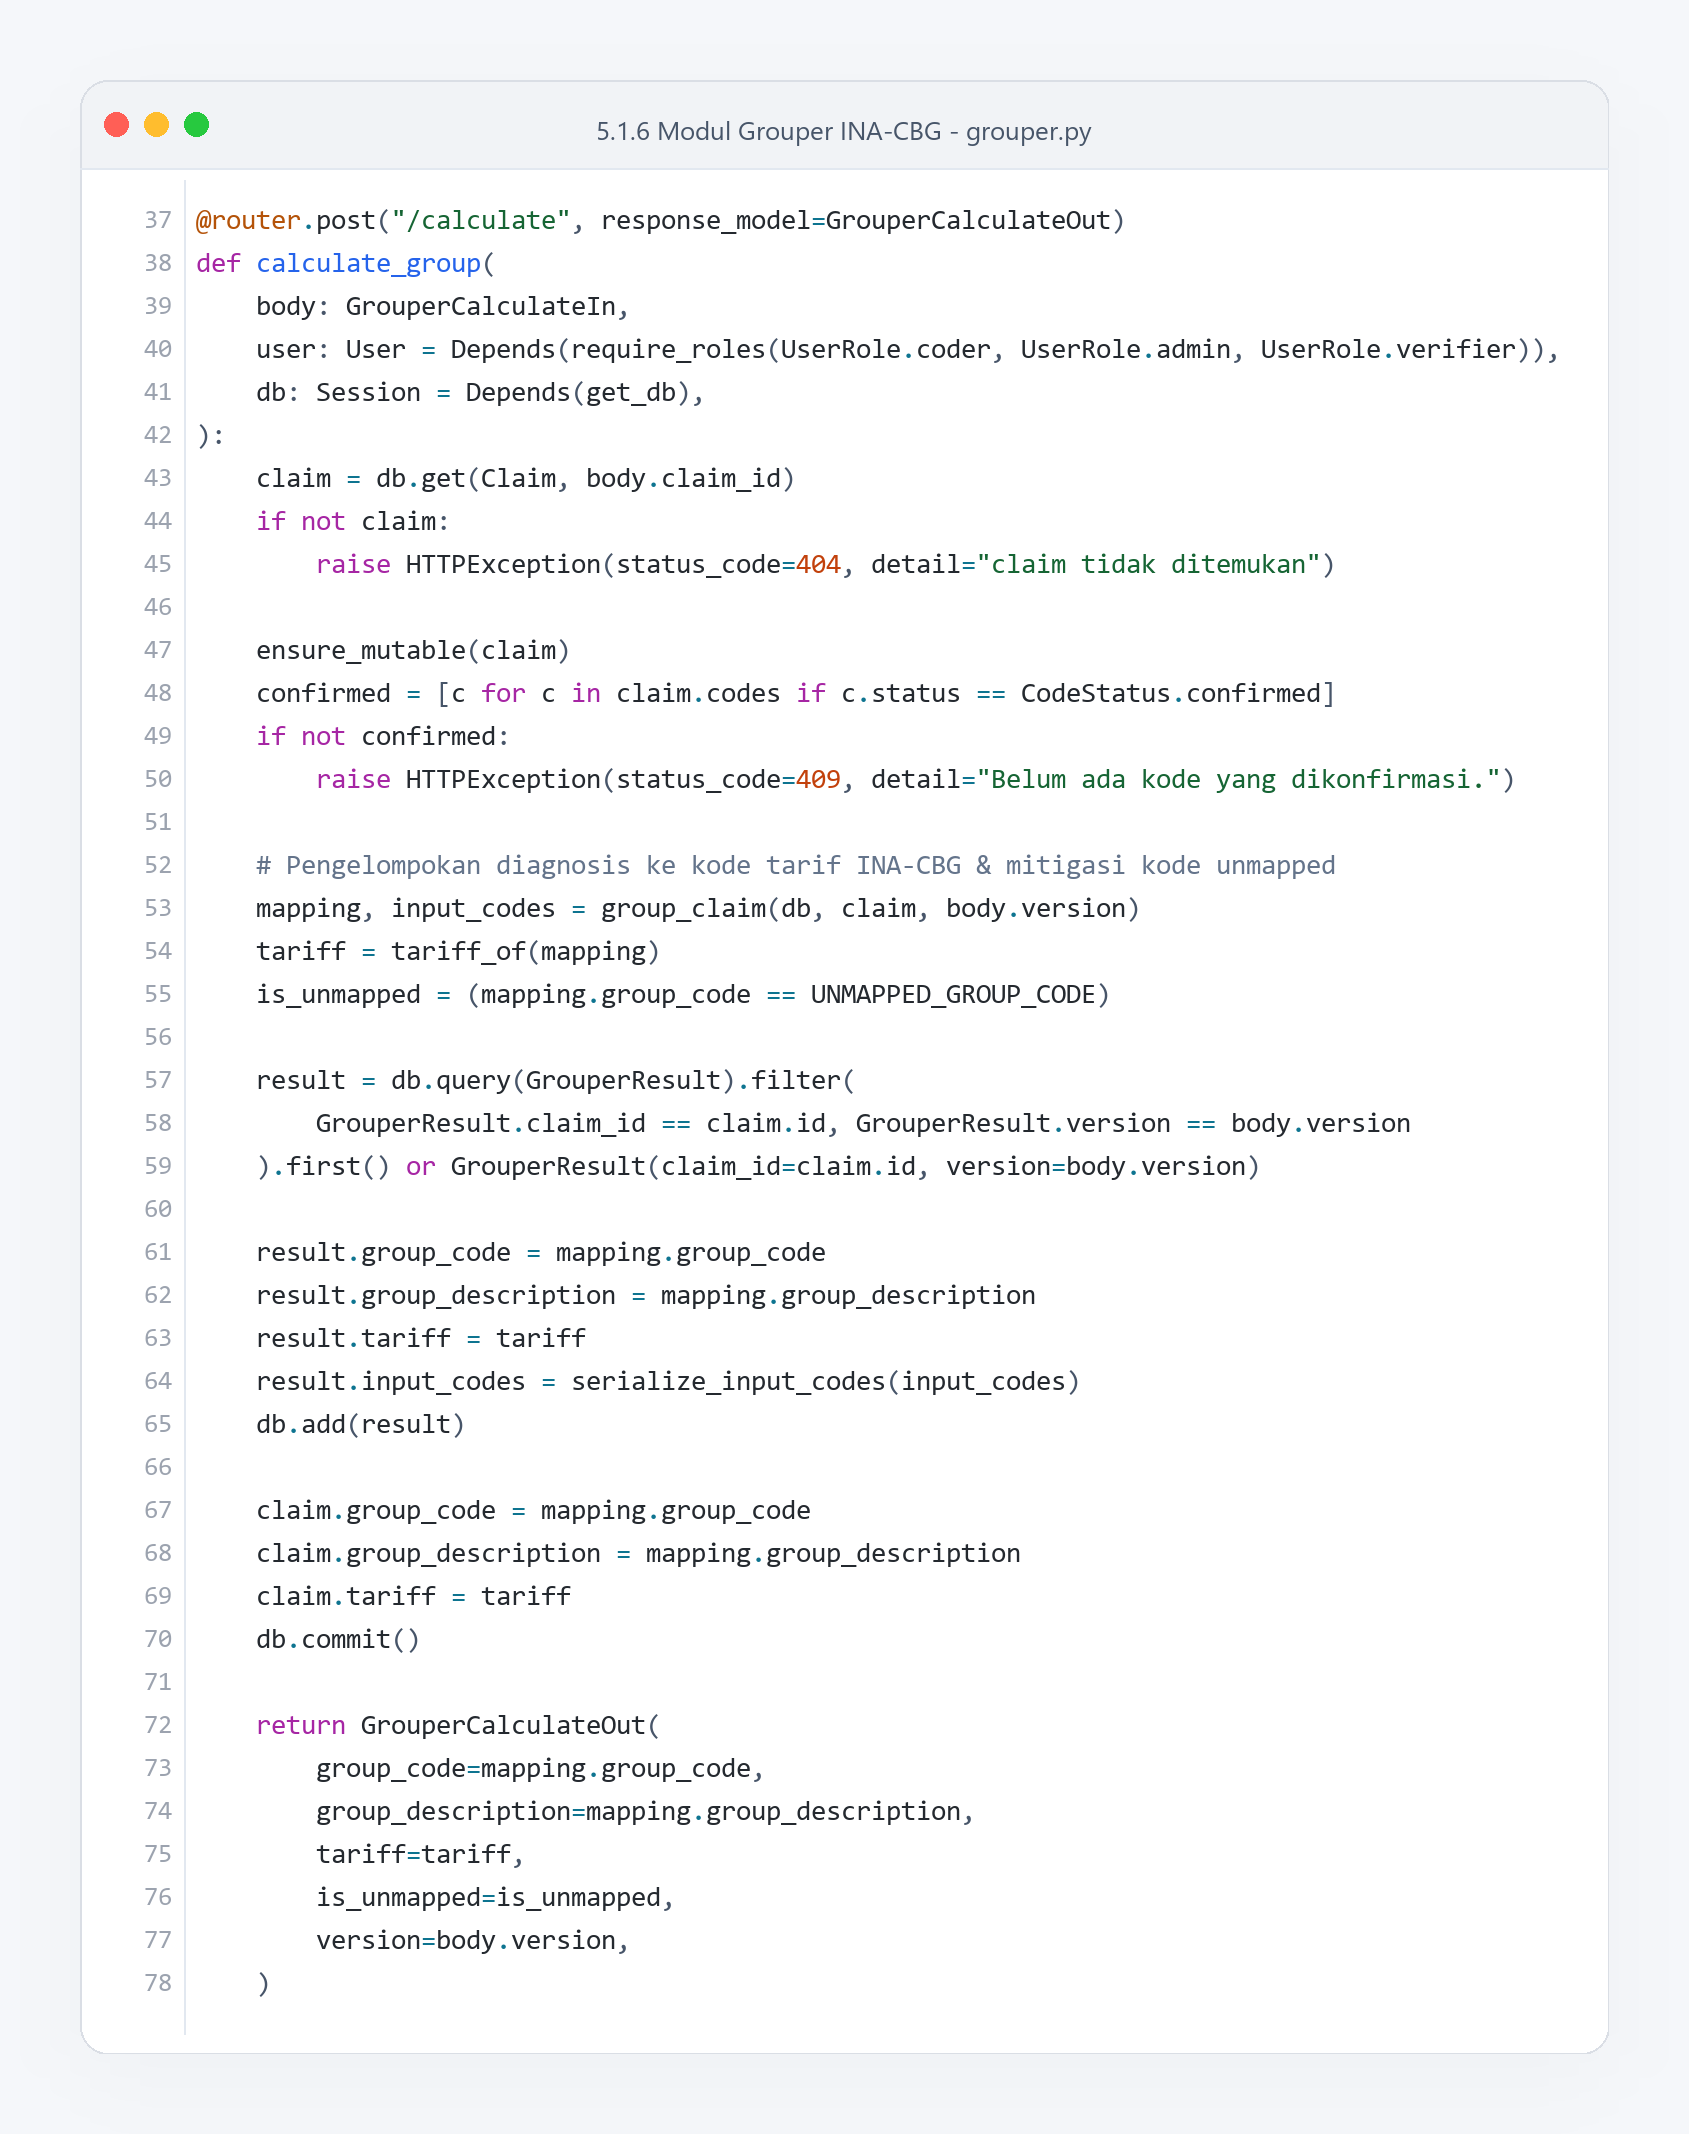
\includegraphics[width=10.5cm]{figure/code/5.1.6_Modul_Grouper_INACBG.png}
  \caption{Implementasi Mesin Perhitungan Grouper dan Estimasi Tarif INA-CBG}\label{fig:impl-code-grouper}
\end{figure}

Gambar~\ref{fig:impl-code-grouper} menampilkan fungsi calculate\_group() pada endpoint POST /calculate. Sebelum kalkulasi dijalankan, sistem memvalidasi bahwa berkas klaim memiliki sekurang-kurangnya satu kode diagnosis yang telah disetujui oleh koder (CodeStatus.confirmed). Pemetaan tarif dijalankan melalui fungsi group\_claim() dengan mencocokkan kode terhadap dataset aturan tarif INA-CBG versi 5.0, memperhitungkan Case-Mix Main Group (CMG) dan tingkat keparahan kasus (Case-Mix Severity Level) berdasarkan keberadaan prosedur tindakan medis yang menyertainya.

Untuk mencegah terjadinya kesalahan klaim biaya yang dapat menimbulkan risiko finansial bagi rumah sakit, penulis merancang mekanisme pengamanan isolasi di mana kombinasi kode yang belum memiliki aturan pemetaan resmi dalam data demo akan dialokasikan ke kelompok kasus khusus X-UNMAPPED dengan nilai tarif Rp0 dan penanda is\_unmapped=True. Sistem juga menyertakan peringatan eksplisit bahwa nilai yang muncul merupakan estimasi demo. Hasil kalkulasi kelompok kasus dan estimasi nominal biaya disimpan ke dalam tabel grouper\_results serta diperbarui.

\subsection{Modul Pencarian ICD dan Pemetaan}
Fasilitas penelusuran katalog referensi kode diagnosis dan rekomendasi pemetaan prosedur klinis diimplementasikan pada berkas backend/app/api/v1/icd.py dan backend/app/api/v1/icd\_mapping.py, seperti ditunjukkan pada Gambar~\ref{fig:impl-code-icd-search}.

\begin{figure}[!ht]
  \centering
  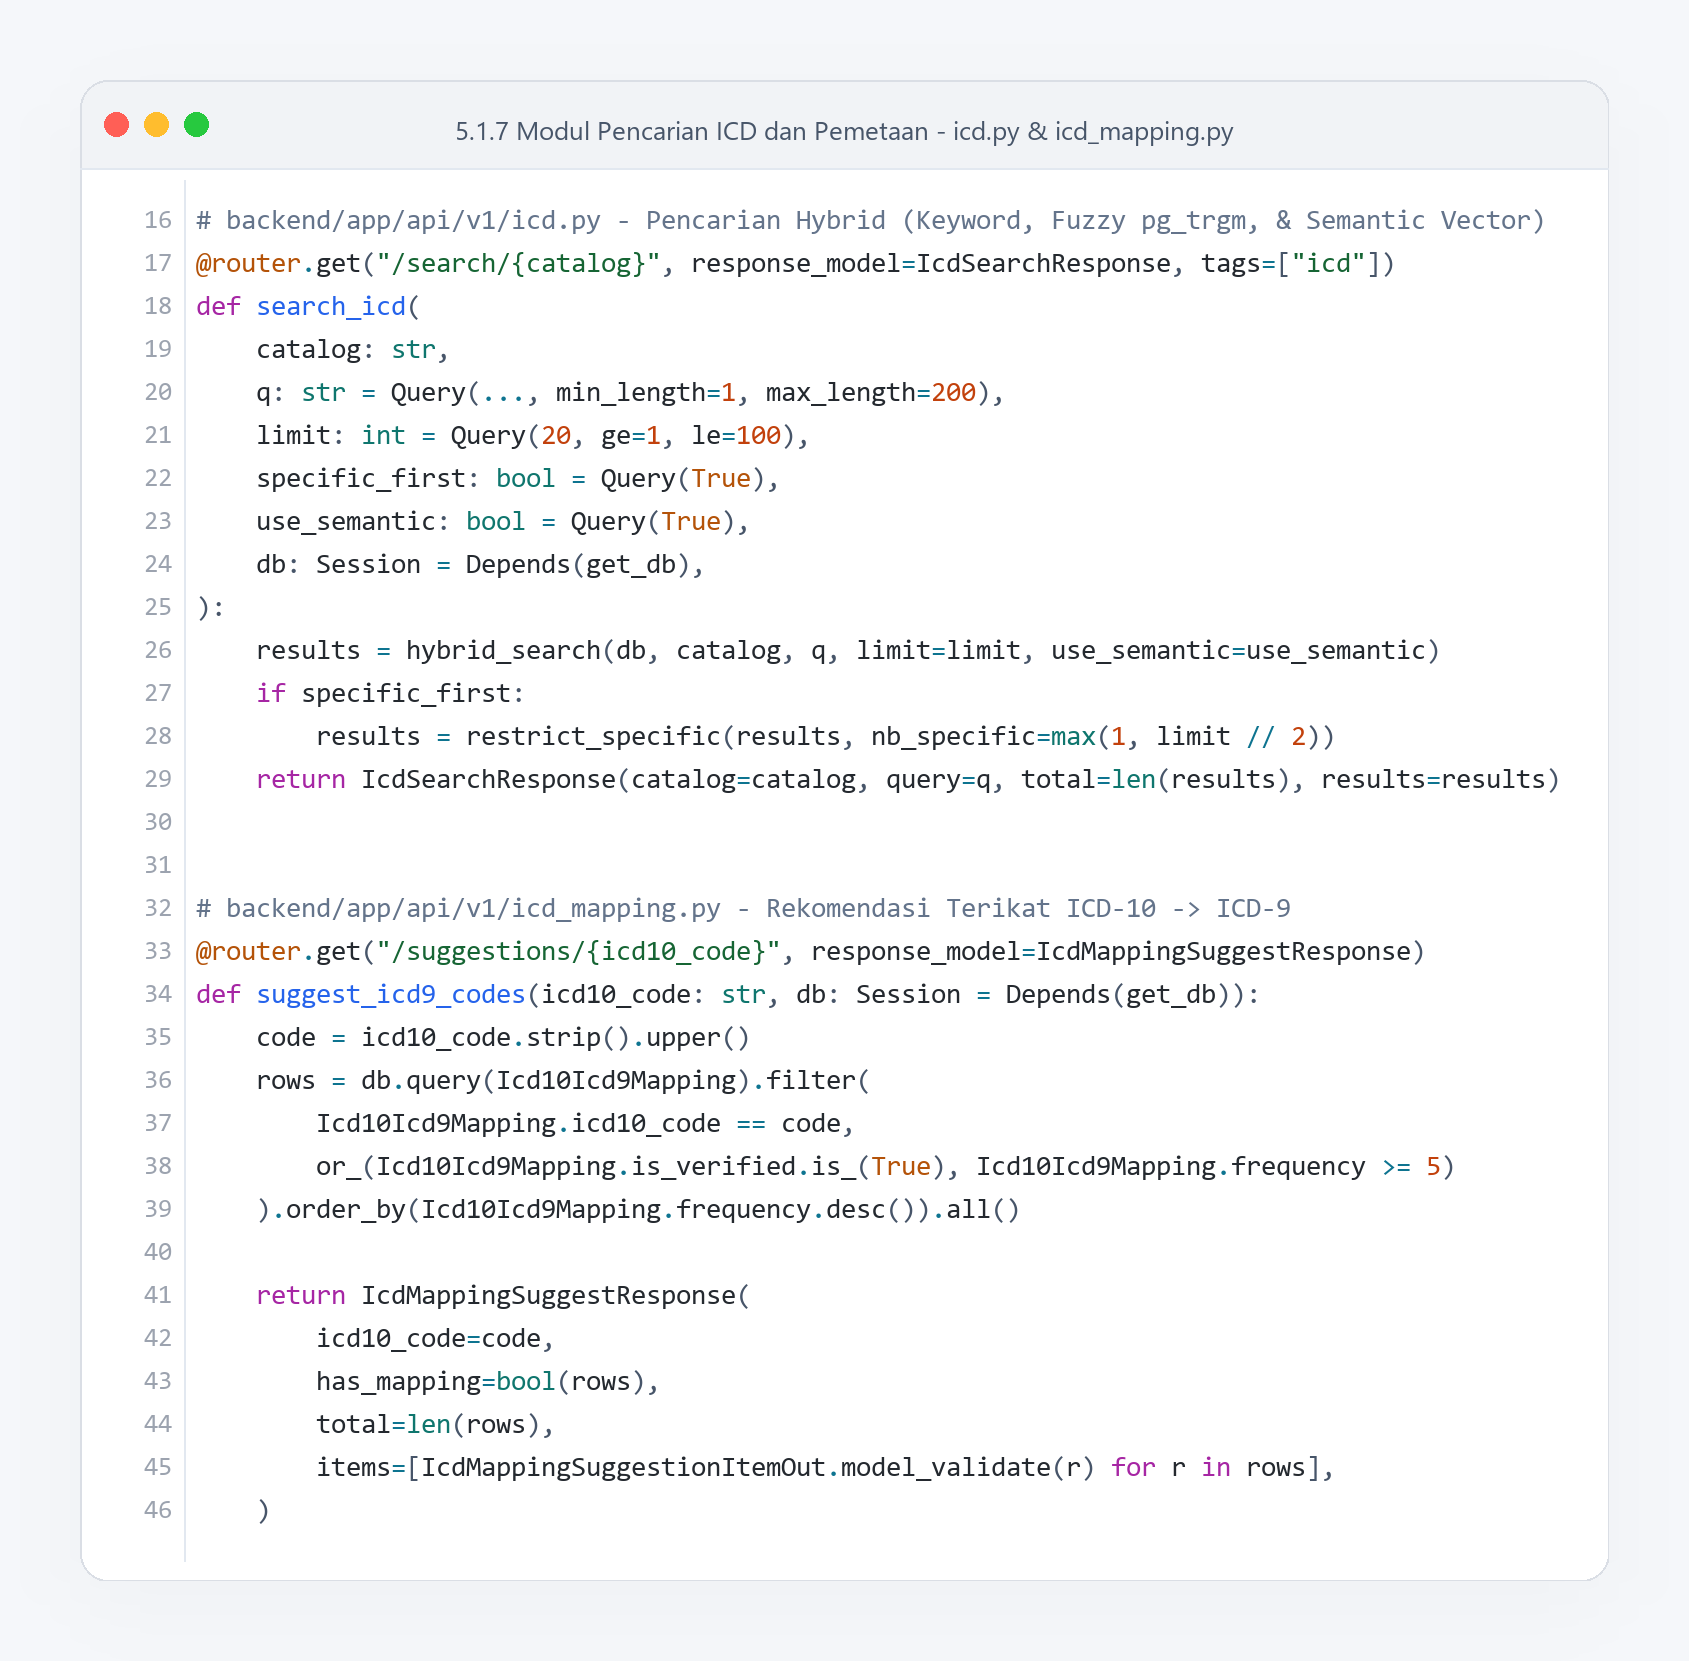
\includegraphics[width=11.5cm]{figure/code/5.1.7_Modul_Pencarian_ICD_dan_Pemetaan.png}
  \caption{Implementasi Pencarian Hibrida Katalog ICD dan Rekomendasi Pemetaan}\label{fig:impl-code-icd-search}
\end{figure}

Gambar~\ref{fig:impl-code-icd-search} menyajikan dua fungsionalitas utama modul pencarian kode. Bagian atas memperlihatkan endpoint GET /search/\{catalog\} pada fungsi search\_icd() yang menjalankan algoritma pencarian hibrida tiga lapis, menggabungkan pencocokan kata kunci eksak, pencarian toleransi salah ketik menggunakan indeks trigram PostgreSQL (pg\_trgm) dengan ambang batas kemiripan di atas 0,3, serta penelusuran semantik berbasis vektor. Algoritma ini memungkinkan koder menemukan kode medis yang tepat meskipun terjadi salah ketik kecil pada nama latin penyakit.

Bagian bawah memperlihatkan fungsi suggest\_icd9\_codes() pada endpoint GET /suggestions/\{icd10\_code\} yang menelusuri data riwayat relasi pemetaan diagnosis ICD-10 terhadap tindakan ICD-9-CM yang telah terverifikasi secara klinis atau memiliki frekuensi kemunculan tinggi di rumah sakit. Fasilitas rekomendasi keterkaitan ini mempermudah koder dalam menentukan tindakan medis komplementer tanpa harus menelusuri ribuan kode prosedur satu per satu.

\subsection{Modul Verifikasi}
Alur kerja pemeriksaan dan penetapan persetujuan berkas klaim oleh petugas verifikator rumah sakit diimplementasikan pada berkas backend/\-app/\-api/\-v1/\-verification.py, sebagaimana disajikan pada Gambar~\ref{fig:impl-code-verify}.

\begin{figure}[!ht]
  \centering
  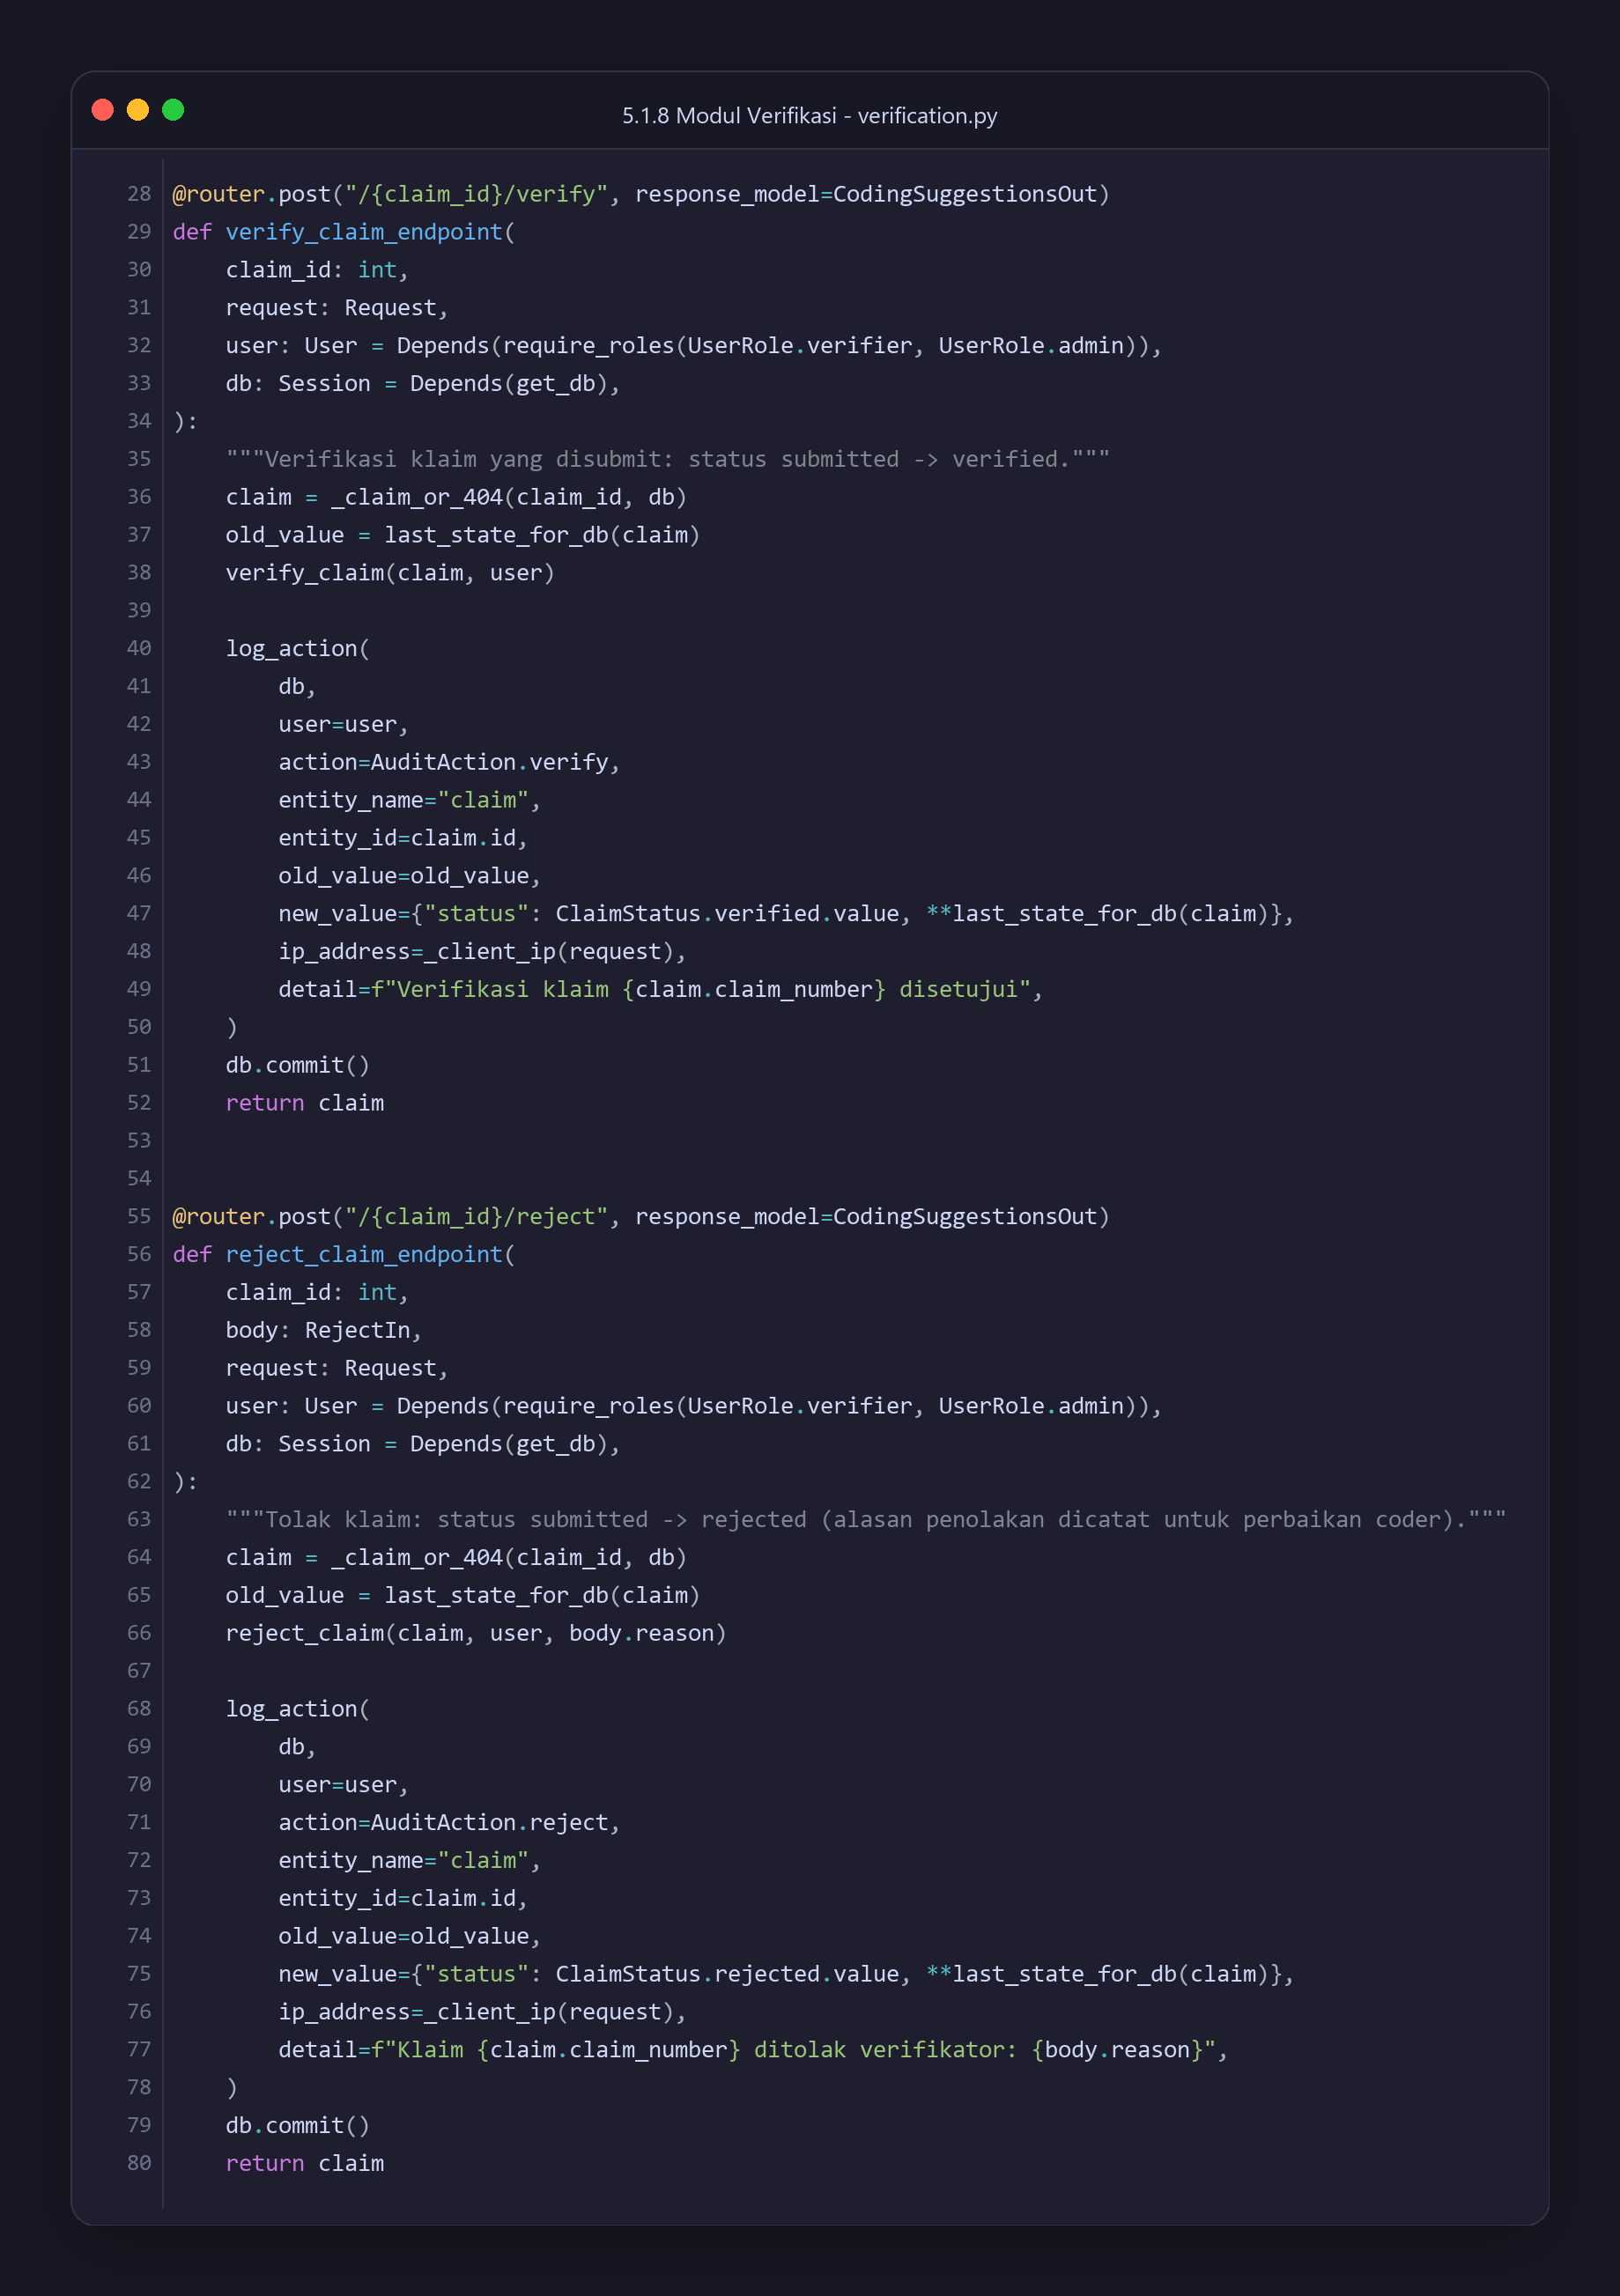
\includegraphics[width=9.5cm]{figure/code/5.1.8_Modul_Verifikasi.png}
  \caption{Implementasi Endpoint Persetujuan dan Penolakan Berkas Verifikator}\label{fig:impl-code-verify}
\end{figure}

Gambar~\ref{fig:impl-code-verify} memperlihatkan implementasi dua endpoint utama verifikasi yang dilindungi hak akses peran verifikator dan admin. Penulis menerapkan prinsip pemisahan tugas (separation of duties) di mana koder yang menginput klaim dilarang melakukan verifikasi sendiri terhadap berkas tersebut guna mencegah potensi bias dan manipulasi data klaim.

Fungsi verify\_claim\_endpoint() menangani persetujuan berkas klaim yang berstatus submitted, memperbarui status berkas menjadi verified, mencatat stempel waktu serta identitas verifikator pada kolom verified\_by\_id, dan merekam peristiwa persetujuan ke log audit. Sebaliknya, fungsi reject\_claim\_endpoint() menangani penolakan berkas klaim yang tidak memenuhi kelengkapan medis atau terdapat ketidaksesuaian diagnosis. Sistem mewajibkan pencantuman alasan penolakan secara tertulis (body.reason) dan mengembalikan status berkas klaim menjadi rejected agar staf koder dapat menelaah catatan kekurangan tersebut dan segera melakukan perbaikan koding klinis.

\subsection{Modul Audit dan Metrik}
Pencatatan rekam jejak aktivitas operasional serta penyajian ringkasan metrik kinerja sistem diimplementasikan pada berkas backend/app/api/v1/audit.py dan backend/app/api/v1/metrics.py, seperti diperlihatkan pada Gambar~\ref{fig:impl-code-audit-metrics}.

\begin{figure}[!ht]
  \centering
  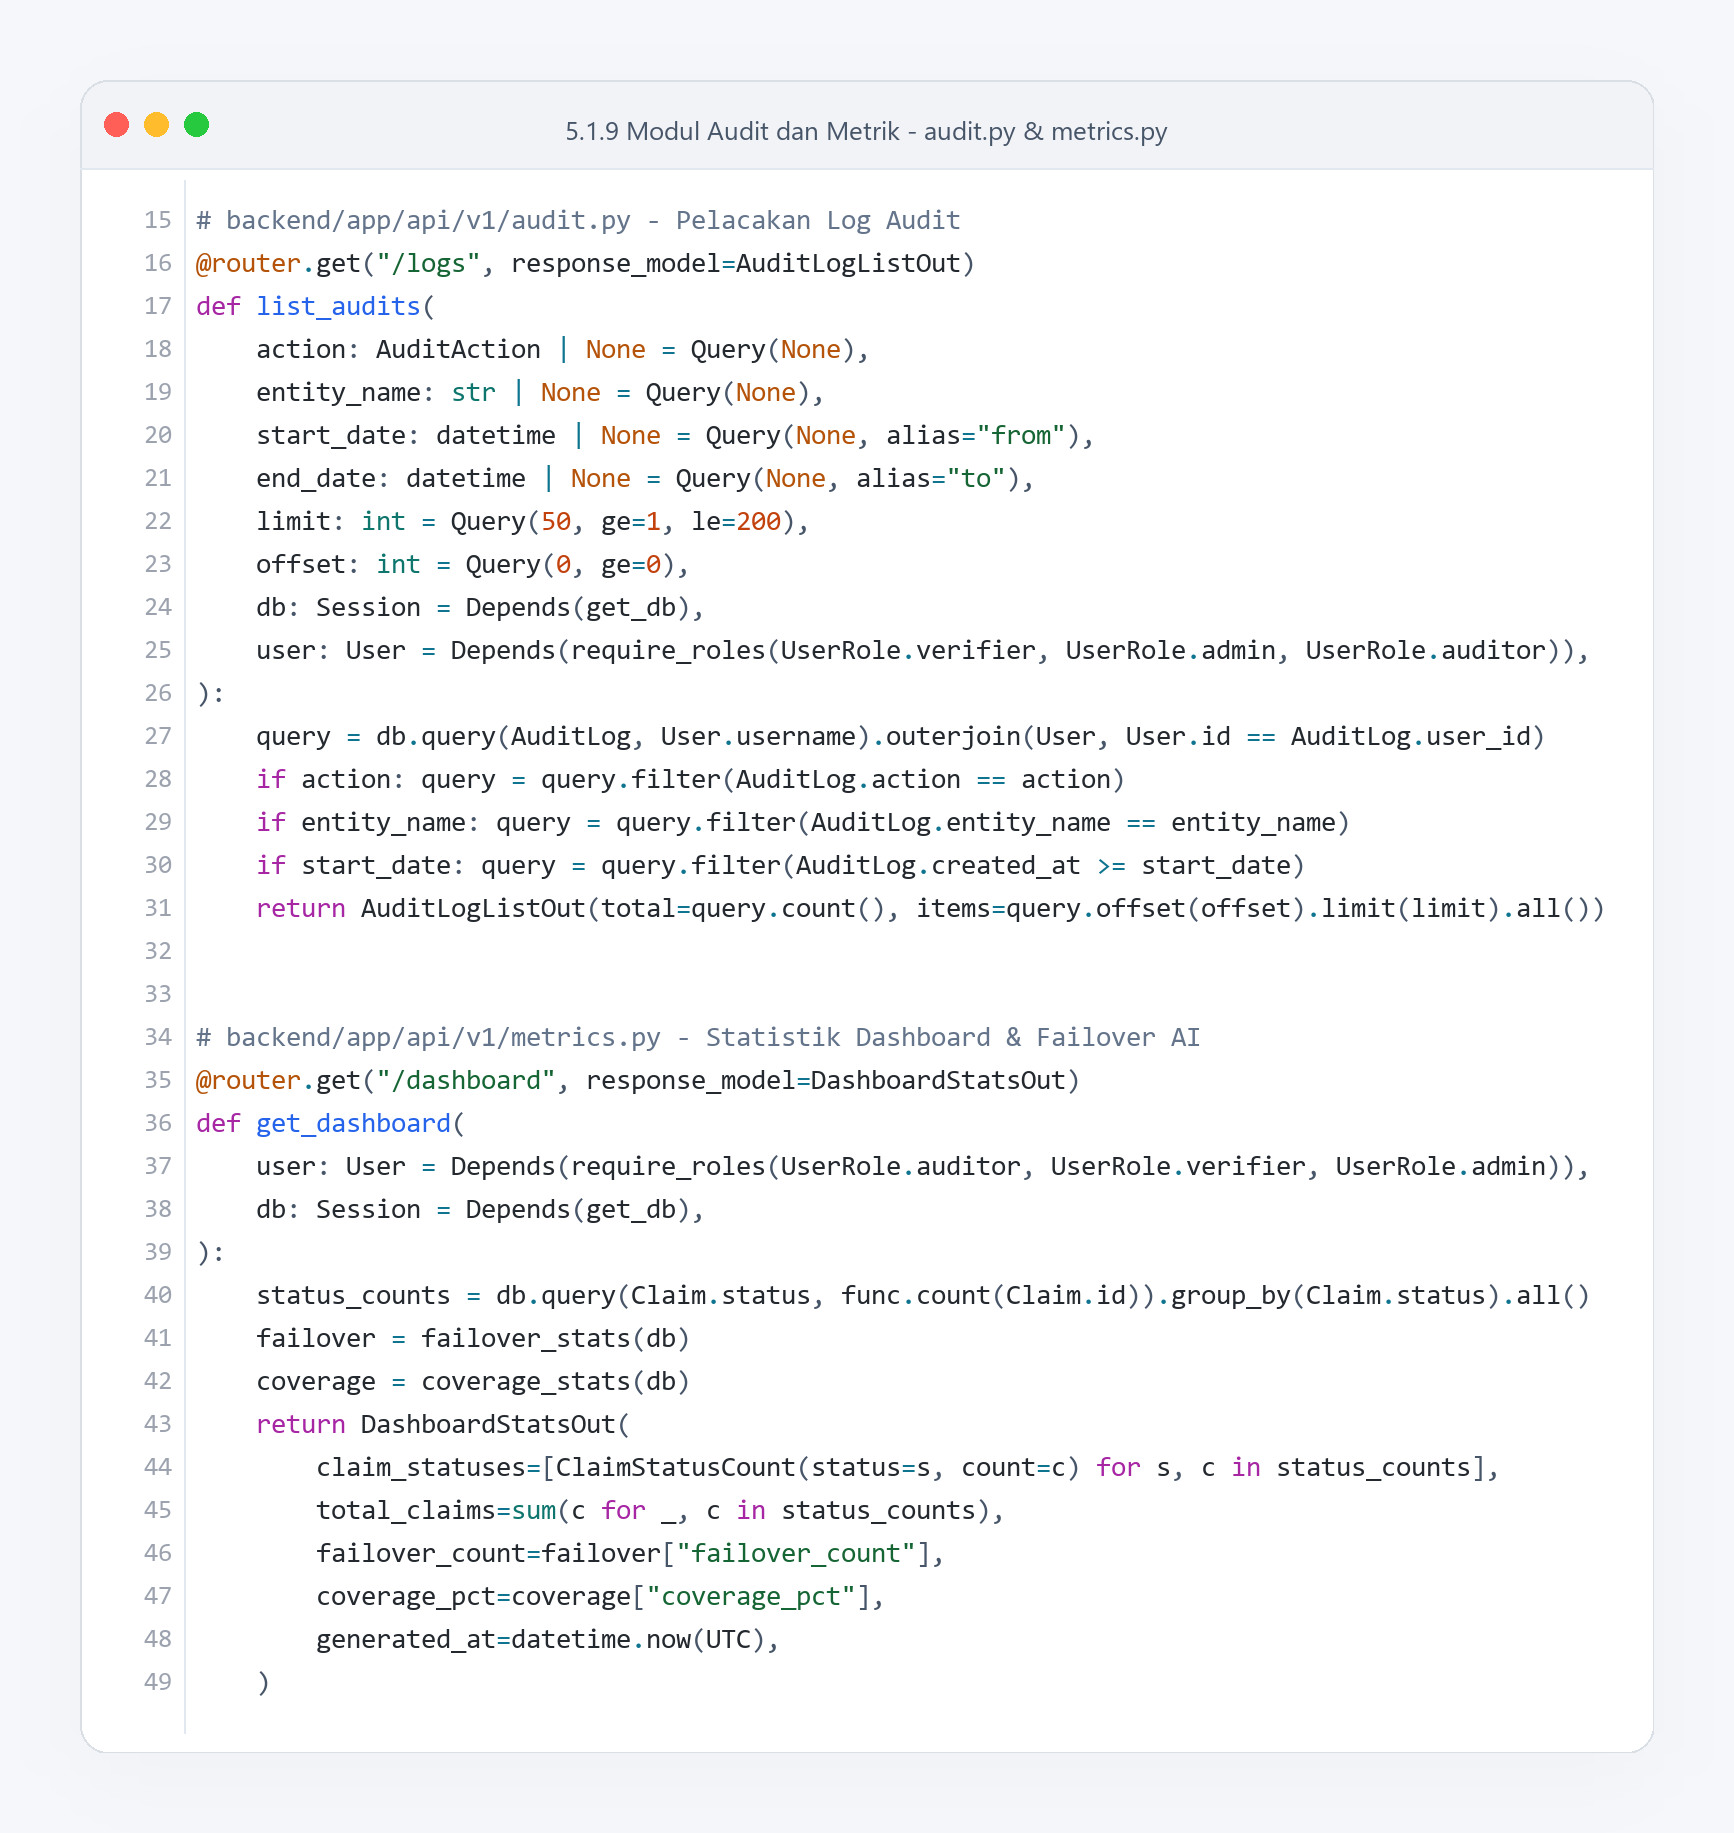
\includegraphics[width=11.5cm]{figure/code/5.1.9_Modul_Audit_dan_Metrik.png}
  \caption{Implementasi Penelusuran Jejak Audit dan Dasbor Analitik Kinerja}\label{fig:impl-code-audit-metrics}
\end{figure}

Gambar~\ref{fig:impl-code-audit-metrics} menguraikan dua fungsi analitik pengawasan sistem. Fungsi list\_audits() menyediakan fasilitas penelusuran rekaman jejak audit dengan parameter penyaring fleksibel mencakup jenis tindakan, nama entitas transaksi, serta rentang tanggal pelaksanaan aktivitas. Kueri dijalankan secara efisien dengan memanfaatkan indeks komposit pada stempel waktu dan menggabungkan tabel pengguna untuk menampilkan identitas akun pelaksana aksi.

Di sisi lain, fungsi get\_dashboard() menghitung agregasi statistik operasional rumah sakit secara langsung melalui kueri SQL analitik, meliputi rekapitulasi jumlah klaim per status, akumulasi insiden pengalihan model kecerdasan buatan (failover\_count), jumlah dokumen pindaian yang memerlukan review manual OCR, serta persentase cakupan keberhasilan pemetaan tarif grouper. Dasbor ini membantu pihak manajemen rumah sakit dan auditor medis dalam memantau tren operasional koding harian secara objektif.

\subsection{Indikator Koneksi}
Komponen pemantauan ketersediaan peladen backend secara waktu nyata diimplementasikan pada antarmuka klien menggunakan berkas frontend/src/ConnectionStatus.jsx, sebagaimana diilustrasikan pada Gambar~\ref{fig:impl-code-conn-status}.

\begin{figure}[!ht]
  \centering
  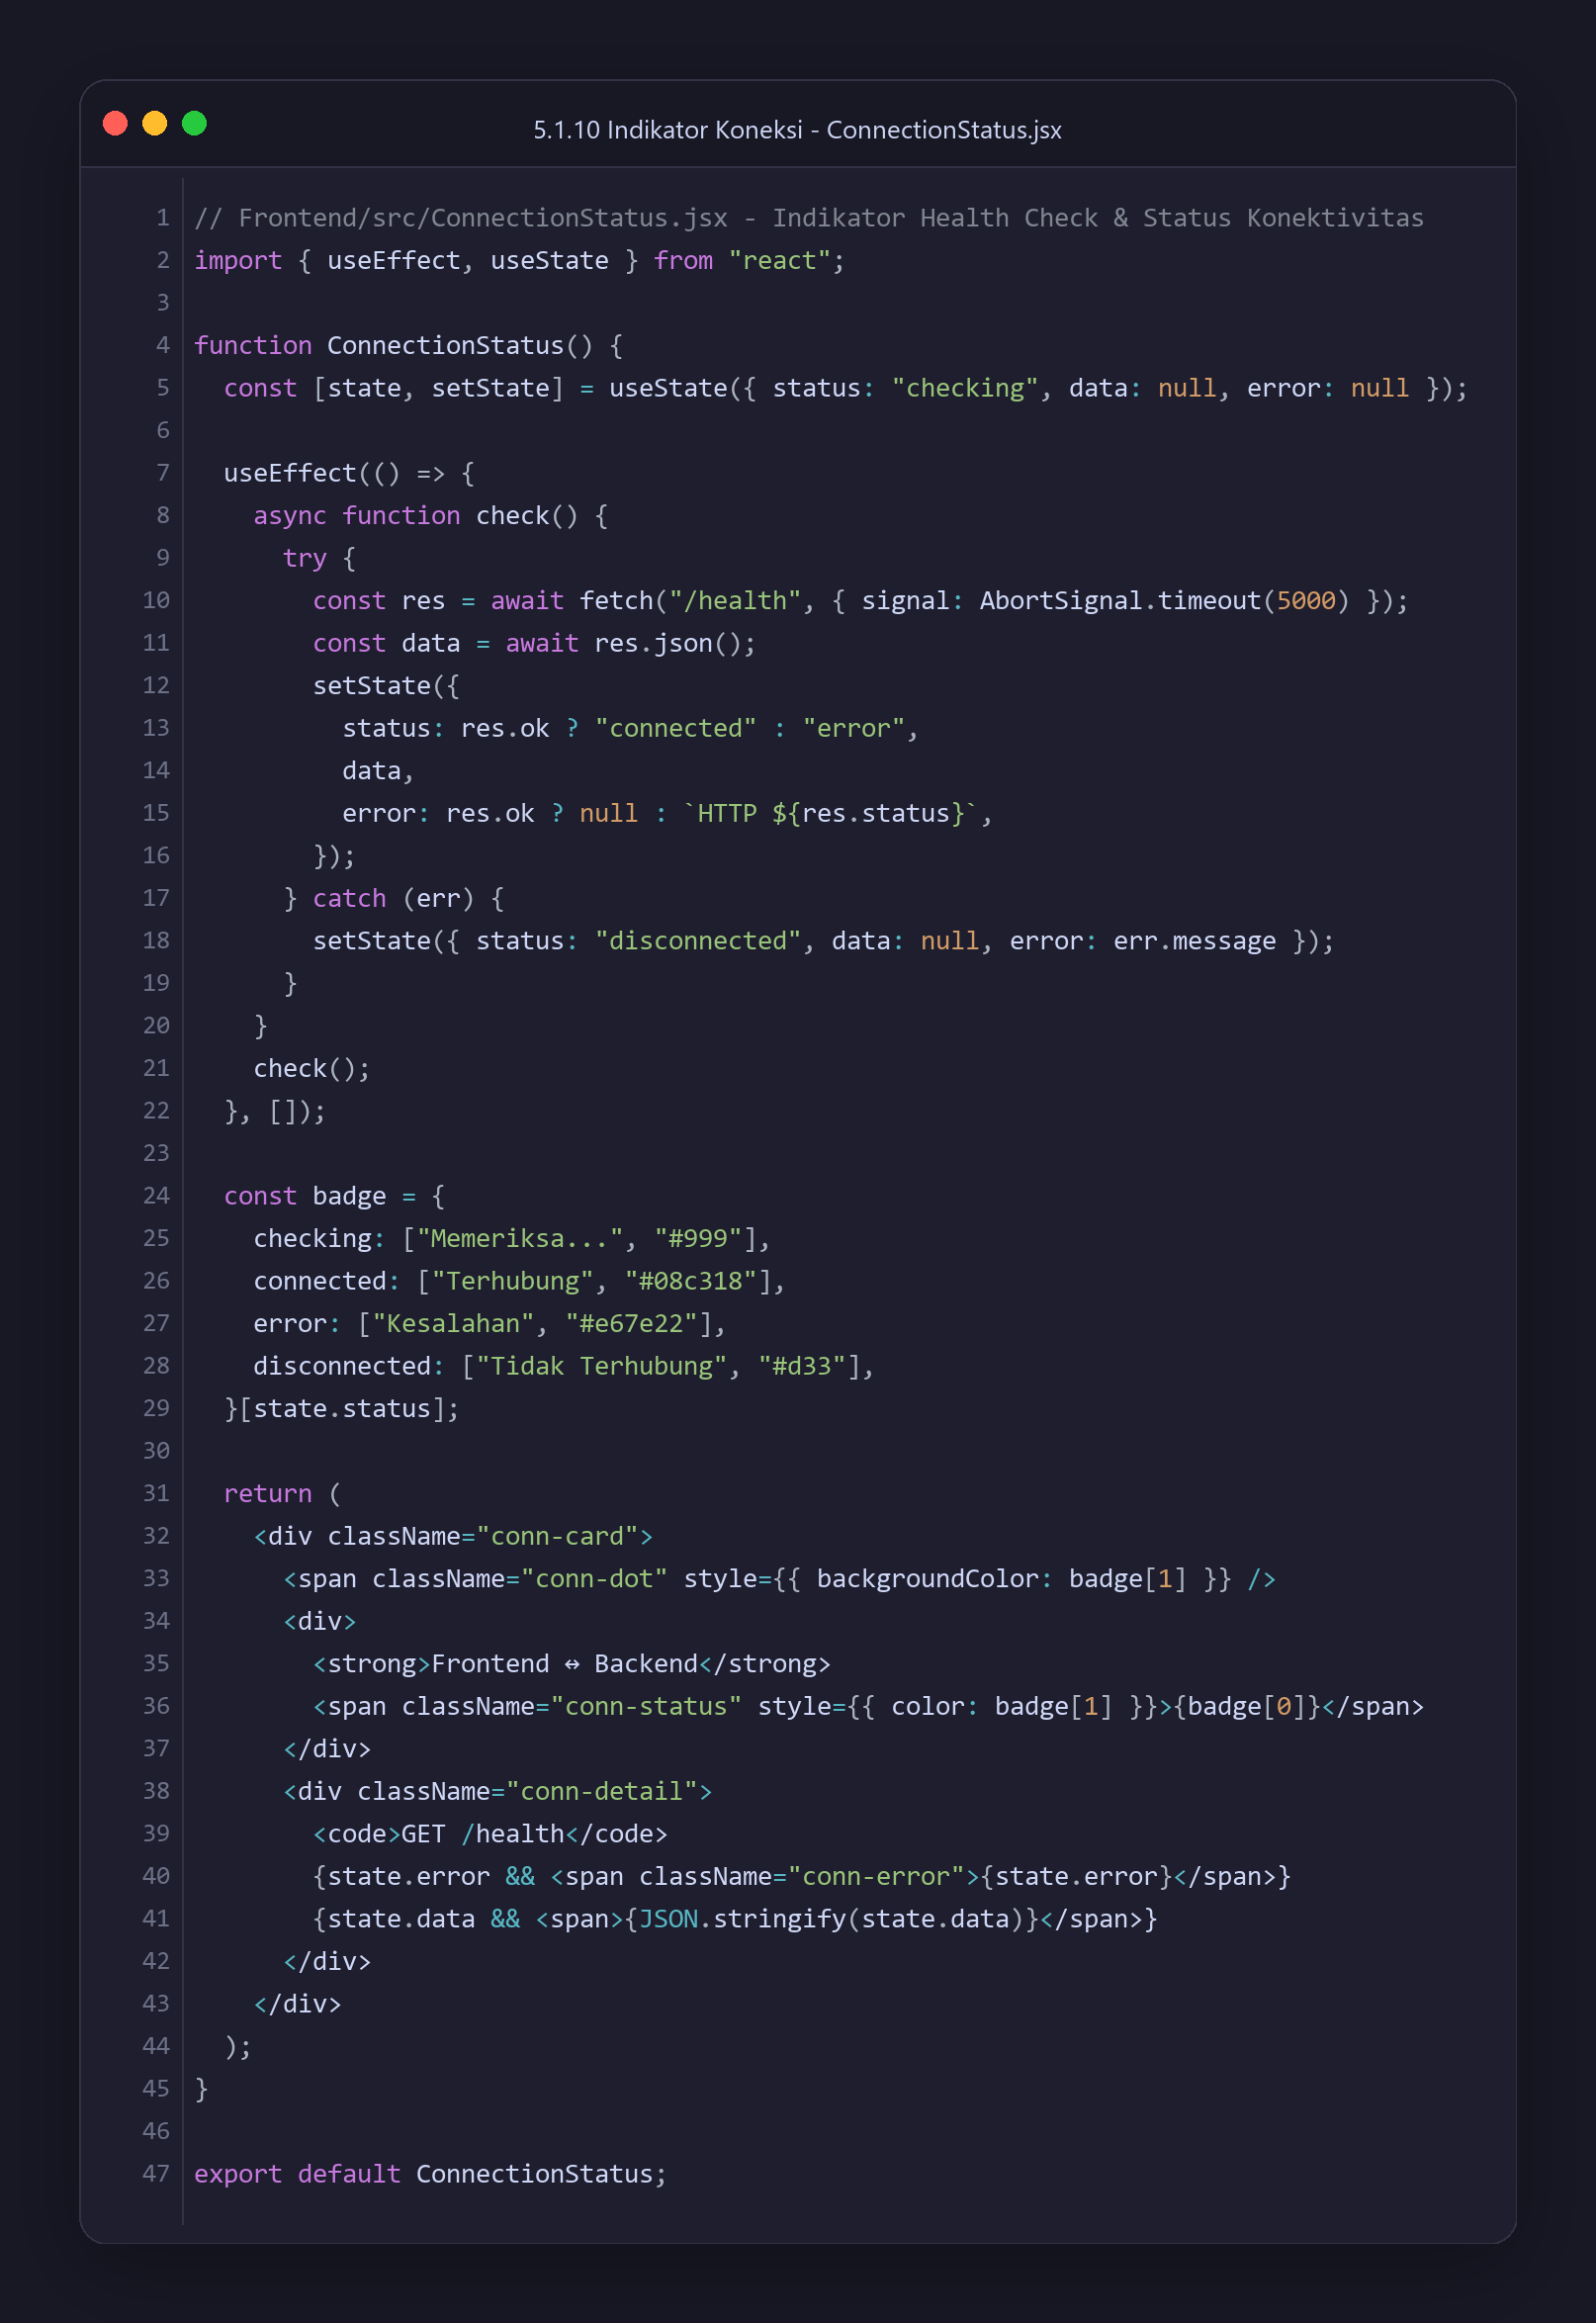
\includegraphics[width=9.5cm]{figure/code/5.1.10_Indikator_Koneksi.png}
  \caption{Implementasi Komponen Klien Pemantau Ketersediaan Layanan Peladen}\label{fig:impl-code-conn-status}
\end{figure}

Gambar~\ref{fig:impl-code-conn-status} menyajikan komponen React ConnectionStatus yang secara berkala memeriksa keterhubungan jaringan ke peladen backend melalui pemanggilan fetch('/health'). Penulis melengkapi komponen ini dengan pengendali batas waktu koneksi menggunakan AbortSignal.timeout(5000) untuk mencegah proses penungguan yang menggantung ketika terjadi latensi jaringan atau peladen sedang mengalami beban kerja puncak.

Status konektivitas dikelompokkan ke dalam empat kondisi visual: checking, connected, error, dan disconnected, lengkap dengan indikator warna titik status dan kartu informasi diagnostik yang menampilkan status respons peladen serta penyedia model kecerdasan buatan yang sedang aktif beroperasi (Google Gemini atau cadangan OpenRouter). Komponen ini memberikan kepastian informasi kepada petugas koder rumah sakit mengenai kesiapan infrastruktur backend sebelum memulai proses pengunggahan berkas atau koding klaim.

\subsection{Hasil Pengujian Blackbox Testing}
Pengujian sistem dilakukan menggunakan metode \textit{blackbox testing} terhadap fungsionalitas utama pada setiap modul yang telah dikembangkan. Pengujian ini bertujuan untuk memastikan bahwa seluruh fungsi sistem merespons masukan pengguna dengan hasil yang sesuai dengan spesifikasi kebutuhan perangkat lunak yang telah dirancang pada Bab IV. Pelaksanaan pengujian berlandaskan (\textit{ground-based}) dan divalidasi silang terhadap rangkaian pengujian otomatis (\textit{automated test suite}) pada direktori backend/tests.

\subsubsection{Identitas dan Parameter Lingkungan Pengujian}
Sebelum pelaksanaan pengujian, ditetapkan identitas dokumen serta spesifikasi lingkungan eksekusi pengujian sebagai berikut:
\begin{itemize}[leftmargin=1.5em, itemsep=1pt]
  \item Nama Proyek / Sistem: INA-CBG Coding Assistant.
  \item Lingkup Fitur yang Diuji: Modul Autentikasi, Modul Otorisasi (\textit{Role-Based Access Control}/RBAC), Modul Manajemen Klaim, Modul Koding Klinis \& AI, Modul Grouper INA-CBG, Modul Verifikasi Klaim, dan Modul Audit Trail.
  \item Penguji (\textit{Tester}): Tim Pengembang dan Automated QA Test Runner (pytest / httpx).
  \item Tanggal Pengujian: 23 Oktober 2026.
  \item Spesifikasi Lingkungan: Python 3.11+, FastAPI (ASGI), PostgreSQL 15+ (ekstensi pg\_trgm), Celery Worker, Redis Cache.
\end{itemize}

\subsubsection{Rancangan dan Hasil Kasus Uji (Test Case)}
Rincian rancangan skenario kasus uji, data uji yang digunakan, langkah-langkah pengujian, hasil yang diharapkan, hasil aktual, status kelulusan, serta rujukan berkas pengujian otomatis disajikan pada Tabel~\ref{tab:blackbox-testing}.

\begin{scriptsize}
\setlength{\tabcolsep}{1.5pt}
\begin{longtable}{|>{\raggedright\arraybackslash}p{1.3cm}|>{\raggedright\arraybackslash}p{1.9cm}|>{\raggedright\arraybackslash}p{1.8cm}|>{\raggedright\arraybackslash}p{2.1cm}|>{\raggedright\arraybackslash}p{1.8cm}|>{\raggedright\arraybackslash}p{1.5cm}|>{\centering\arraybackslash}p{0.8cm}|>{\raggedright\arraybackslash}p{2.2cm}|}
\caption{Tabel Kasus Uji Blackbox Testing}\label{tab:blackbox-testing}\\
\hline
ID Test Case & Modul \& Skenario & Data Uji (Test Data) & Langkah Pengujian & Hasil Diharapkan & Hasil Aktual & Status & Python Code Test \\
\hline
\endfirsthead
\hline
ID Test Case & Modul \& Skenario & Data Uji (Test Data) & Langkah Pengujian & Hasil Diharapkan & Hasil Aktual & Status & Python Code Test \\
\hline
\endhead
\hline
\endfoot
TC-AUTH-\newline 001 & Autentikasi: Login kredensial benar (admin) & Username: "admin"\newline Password:\newline "admin12345" & 1. Kirim POST /api/v1/\newline auth/login\newline 2. Sertakan JSON kredensial valid\newline 3. Evaluasi respons & Token JWT dan data pengguna dikembalikan (HTTP 200 OK) & Token JWT dan data pengguna dikembalikan & Lulus & tests/\newline test\_api\_e2e.py\newline (TestAuthE2E,\newline helper \_login) \\ \hline
TC-AUTH-\newline 002 & Autentikasi: Login kata sandi salah & Username: "admin"\newline Password:\newline "salah123" & 1. Kirim POST /api/v1/\newline auth/login\newline 2. Masukkan sandi salah\newline 3. Cek proteksi sistem & Error 401 Unauthorized ("detail": "Incorrect password") & Error 401 Unauthorized & Lulus & tests/\newline test\_api\_e2e.py\newline (test\_wrong\_\newline password\_401) \\ \hline
TC-AUTH-\newline 003 & Autentikasi: Akses endpoint tanpa token & Header: Tanpa Authorization Bearer & 1. Panggil GET /api/v1/\newline auth/me atau klaim\newline 2. Tanpa Bearer Token\newline 3. Amati middleware & Error 401 Unauthorized ("detail": "Not authenticated") & Error 401 Unauthorized & Lulus & tests/\newline test\_api\_e2e.py\newline (test\_me\_\newline requires\_token) \\ \hline
TC-AUTH-\newline 004 & Otorisasi: Coder akses endpoint verifikasi & Token: Role "coder"\newline Endpoint: POST /api/v1/\newline claims/\{id\}/\newline verify & 1. Login akun koder\newline 2. Kirim aksi verifikasi ke endpoint verifikator\newline 3. Evaluasi respons RBAC & Error 403 Forbidden (Hanya role verifier yang diizinkan) & Error 403 Forbidden & Lulus & tests/\newline test\_claim\_flow.py\newline (test\_coder\_\newline cannot\_verify) \\ \hline
TC-CLM-\newline 001 & Klaim: Unggah klaim berkas valid (PDF) & Berkas: rasa.pdf,\newline Form: nomor klaim, SEP, diagnosis & 1. Siapkan file PDF \& metadata valid\newline 2. Kirim multipart ke POST /api/v1/\newline claims/upload\newline 3. Cek status berkas & Klaim pending + dokumen tersimpan (HTTP 201 Created) & Klaim pending + dokumen tersimpan & Lulus & tests/\newline test\_api\_e2e.py\newline (test\_full\_\newline pipeline) \\ \hline
TC-CLM-\newline 002 & Klaim: Unggah berkas melebihi batas ukuran & File PDF dummy $>$ 15 MB (melebihi batas sistem) & 1. Pilih berkas melebihi kuota upload\newline 2. Kirim ke POST /api/v1/\newline claims/upload\newline 3. Cek respons sistem & Error 413 Payload Too Large (Ukuran file melebihi batas) & Error 413 Payload Too Large & Lulus & endpoints/\newline claims.py \&\newline core/config.py \\ \hline
TC-CLM-\newline 003 & Klaim: Duplikasi nomor klaim & claim\_number:\newline "CLM-E2E-001"\newline (sudah terdaftar) & 1. Unggah nomor klaim yang sudah terdaftar\newline 2. Cek integritas unique constraint & Error 409 Conflict (Nomor klaim sudah terdaftar) & Error 409 Conflict & Lulus & tests/\newline test\_api\_e2e.py\newline (test\_duplicate\_\newline claim\_409) \\ \hline
TC-COD-\newline 001 & Koding: Konfirmasi kode tanpa claim\_code\_id & Payload: action:\newline confirm,\newline is\_primary: true & 1. Kirim PUT /api/v1/\newline coding/\{id\}/codes\newline 2. Abaikan atribut claim\_code\_id\newline 3. Cek validasi skema & Error 422 Unprocessable Entity & Error 422 & Lulus & schemas/\newline coding.py \&\newline tests/\newline test\_api\_e2e.py \\ \hline
TC-COD-\newline 002 & Koding: Tambah kode manual tanpa katalog/kode & Payload: action: add, reason: manual & 1. Kirim PUT /api/v1/\newline coding/\{id\}/codes\newline 2. Kosongkan katalog \& kode\newline 3. Cek validasi skema & Error 422 Unprocessable Entity & Error 422 & Lulus & schemas/\newline coding.py \&\newline tests/\newline test\_api\_e2e.py \\ \hline
TC-COD-\newline 003 & Koding: Analisis AI teks klinis kosong/tanpa konten & Resume: string kosong "" / tanpa karakter teks & 1. Analisis kode AI pada teks resume kosong\newline 2. Amati parser AI \& mekanisme failover & Respons tidak menghasilkan kode / rekomendasi kosong (codes: []) & Sesuai & Lulus & tests/\newline test\_ai\_provider.py\newline \& worker\_\newline robustness.py \\ \hline
TC-GRP-\newline 001 & Grouper: Kalkulasi dengan kode tidak dikenal & Diagnosis primer:\newline "ZZZ.99" (tidak ada di master ICD) & 1. Masukkan diagnosis primer invalid\newline 2. Kirim POST /api/v1/\newline grouper/calculate\newline 3. Cek respon grouper & Error 422 Unprocessable Entity & Error 422 & Lulus & tests/\newline test\_grouper.py\newline (TestCalculate\newline Grouper) \\ \hline
TC-GRP-\newline 002 & Grouper: Kalkulasi kode dikenal tanpa mapping & Diagnosis ICD-10 valid namun belum ada aturan tarif & 1. Tetapkan diagnosis tanpa mapping aktif\newline 2. Kirim POST /api/v1/\newline grouper/calculate\newline 3. Evaluasi penanganan & Grup X-UNMAPPED, tarif 0, is\_unmapped = true + demo & Sesuai & Lulus & tests/\newline test\_grouper.py\newline (TestUnmapped\newline Fallback) \\ \hline
TC-VER-\newline 001 & Verifikasi: Tolak klaim tanpa alasan & Payload: reason\newline kosong "" & 1. Verifikator eksekusi POST /api/v1/\newline claims/\{id\}/reject\newline 2. Alasan dikosongkan\newline 3. Cek respons API & Error 422 (alasan penolakan wajib disertakan) & Error 422 & Lulus & tests/\newline test\_claim\_flow.py\newline (test\_reject\_\newline requires\_reason) \\ \hline
TC-VER-\newline 002 & Verifikasi: Verifikasi klaim berstatus submitted & Klaim submitted,\newline Token: role "verifier" & 1. Tinjau klaim dengan kode terkonfirmasi\newline 2. Kirim POST /api/v1/\newline claims/\{id\}/verify\newline 3. Cek perubahan status & Status menjadi verified + tercatat verifikator & Sesuai & Lulus & tests/\newline test\_claim\_flow.py\newline (test\_happy\_\newline path\_submit) \\ \hline
TC-AUD-\newline 001 & Audit: Aktivitas perubahan kode tercatat di audit & Aksi mutasi kode oleh Coder, Token Admin & 1. Koder mutasi kode klaim\newline 2. Login admin \& buka GET /api/v1/\newline audit/logs\newline 3. Cek rekaman log audit & Tercatat dalam tabel log audit (action, user\_id, claim\_id, detail aksi) & Sesuai (Log tercatat lengkap dan terstruktur) & Lulus & tests/\newline test\_api\_e2e.py\newline \& test\_icd\_\newline search\_audit.py \\ \hline
\end{longtable}
\end{scriptsize}

\subsubsection{Pemetaan Ground Base Terhadap Pengujian Otomatis Python}
Seluruh rancangan skenario pengujian \textit{blackbox} pada Tabel~\ref{tab:blackbox-testing} berlandaskan (\textit{ground-based}) dan tervalidasi secara otomatis melalui rangkaian pengujian unit dan integrasi \textit{end-to-end} pada direktori backend/tests:
\begin{enumerate}[leftmargin=1.5em, itemsep=2pt]
  \item Modul Autentikasi dan Otorisasi (TC-AUTH-001 sampai TC-AUTH-004): Diimplementasikan pada berkas backend/tests/test\_api\_e2e.py (kelas TestAuthE2E) dan backend/tests/test\_claim\_flow.py (fungsi test\_coder\_cannot\_verify). Pengujian menjamin keamanan penerbitan token JWT, penolakan kredensial ilegal (HTTP 401 Unauthorized), proteksi endpoint privat tanpa token, serta isolasi peran pengguna (\textit{Role-Based Access Control}/RBAC dengan HTTP 403 Forbidden) di mana koder tidak diperkenankan mengakses endpoint verifikasi.
  \item Modul Manajemen Klaim (TC-CLM-001 sampai TC-CLM-003): Mengacu pada pengujian alur integrasi penuh pada berkas backend/tests/test\_api\_e2e.py (test\_full\_pipeline dan TestUploadValidation). Pengujian membuktikan keberhasilan pengunggahan berkas PDF multipart secara asinkron (HTTP 201 Created), penolakan berkas melebihi batas ukuran (HTTP 413 Payload Too Large), serta pencegahan duplikasi nomor klaim (HTTP 409 Conflict).
  \item Modul Koding AI dan Rekomendasi (TC-COD-001 sampai TC-COD-003): Divalidasi melalui skema validasi Pydantic pada backend/app/schemas/coding.py, modul parser AI pada backend/tests/test\_ai\_provider.py, serta ketahanan pekerja Celery pada backend/tests/test\_worker\_robustness.py. Sistem terbukti menolak masukan mutasi koding yang tidak lengkap (HTTP 422 Unprocessable Entity) dan mengisolasi catatan medis berteks kosong dengan hasil rekomendasi kosong (codes: []) tanpa menimbulkan galat server.
  \item Modul Grouper INA-CBG (TC-GRP-001 dan TC-GRP-002): Diuji secara komprehensif pada berkas backend/tests/test\_grouper.py (kelas TestCalculateGrouper dan TestUnmappedFallback). Pengujian menjamin proteksi terhadap kode diagnosis asing atau tidak valid (HTTP 422) serta penanganan klaim yang belum memiliki aturan pemetaan tarif melalui status aman X-UNMAPPED bertarif Rp0 disertai peringatan estimasi demo.
  \item Modul Verifikasi dan Audit Trail (TC-VER-001, TC-VER-002, dan TC-AUD-001): Diuji pada berkas backend/tests/test\_claim\_flow.py (skenario penolakan klaim test\_reject\_requires\_reason dan alur persetujuan klaim test\_happy\_path\-\_submit\-\_then\-\_verify) serta berkas backend/\-tests/\-test\_icd\-\_search\-\_audit.py. Pengujian menjamin ketaatan regulasi bahwa penolakan klaim wajib menyertakan alasan yang valid, pemutakhiran jejak verifikator saat klaim disetujui, serta transparansi mutasi data di tabel audit\_logs.
\end{enumerate}

\subsubsection{Kesimpulan Hasil Pengujian Blackbox Testing}
Berdasarkan hasil eksekusi 15 kasus uji pada Tabel~\ref{tab:blackbox-testing}, seluruh skenario uji menghasilkan status Lulus (Pass) dengan tingkat kelulusan 100\%. Respons aktual sistem sepenuhnya konsisten terhadap hasil yang diharapkan berdasarkan spesifikasi kebutuhan perangkat lunak, serta didukung oleh automasi kode pengujian Python pada direktori backend/tests. Hal ini membuktikan bahwa sistem INA-CBG Coding Assistant memiliki tingkat keandalan, integritas data, dan keamanan akses yang tinggi dalam mendukung alur kerja koding medis.

\section{Evaluasi dan Analisis}
Berdasarkan hasil implementasi dan pengujian fungsional, sistem INA-CBG Coding Assistant telah berhasil mewujudkan spesifikasi kebutuhan perangkat lunak yang dirancang. Backend FastAPI, worker Celery, basis data PostgreSQL Supabase, dan penyimpanan Cloudflare R2 terbukti andal dalam mendukung alur koding klaim rumah sakit secara menyeluruh. Evaluasi terhadap pencapaian kebutuhan non-fungsional sistem dijabarkan sebagai berikut:
\begin{enumerate}[leftmargin=1.5em, itemsep=1pt, parsep=0pt]
  \item Keamanan dan Kepatuhan Privasi Data (NF-01): Sistem membatasi hak akses secara ketat melalui autentikasi JWT dan kontrol akses berbasis peran (RBAC) yang terbukti menolak akses ilegal pada kasus uji \texttt{TC-AUTH-003} dan \texttt{TC-AUTH-004}. Selain itu, perlindungan data kesehatan ditegakkan melalui sanitasi otomatis data pribadi pasien (PII) sebelum resume klinis dikirimkan ke model AI eksternal, sesuai mandat UU PDP No. 27 Tahun 2022 dan PMK No. 24 Tahun 2022 \cite{21}, \cite{11}.
  \item Efisiensi Kinerja dan Responsivitas (NF-02): Pemisahan arsitektur antara peladen API FastAPI dan \textit{worker} pemrosesan Celery menjamin antarmuka web dan API tetap responsif saat menerima unggahan berkas (\texttt{TC-CLM-001}) tanpa mengalami pemblokiran alur (\textit{blocking}) akibat proses ekstraksi teks dan inferensi AI yang membutuhkan waktu komputasi intensif.
  \item Keandalan dan Ketahanan Layanan (NF-03): Pengujian ketahanan membuktikan bahwa kegagalan transien pada penyedia AI utama (Google Gemini) dapat diatasi secara mulus melalui mekanisme \textit{auto-failover} ke penyedia cadangan OpenRouter. Di samping itu, antrean tugas Celery dilengkapi batas waktu eksekusi (\textit{time limit}) serta mekanisme \textit{retry} otomatis sehingga tidak menimbulkan proses pemrosesan yang menggantung (\textit{hanging task}).
  \item Keselamatan Klinis dan Pengendalian Risiko (NF-04): Sistem menerapkan prinsip \textit{human-in-the-loop}, rekomendasi AI hanya bertindak sebagai pendukung keputusan klinis yang wajib dikonfirmasi oleh petugas koding sebelum diajukan ke tahap verifikasi klaim. Batasan dataset tarif demo diisolasi secara aman menggunakan status \texttt{X-UNMAPPED} bertarif Rp0 (\texttt{TC-GRP-002}) disertai peringatan eksplisit ``estimasi demo'', sehingga sistem tidak berpotensi menimbulkan kesalahan klaim finansial. Untuk validitas operasional penuh, integrasi dataset resmi Kementerian Kesehatan dan evaluasi akurasi terhadap standar emas (\textit{gold standard}) koding medis menjadi prioritas.
\end{enumerate}
